\documentclass[a4paper,10pt,oneside, fleqn]{article}
% Druckbereich: \areaset[BCOR]{textwidth}{textheight}
% BCOR ist "Binding Correction", also wieviel Innenrand verloren geht
% A4 hat 297mm x 210mm
% wenn keine Marginalien, dann ist Breite 15cm vielleicht besser
%\areaset[0cm]{15cm}{25cm}


\usepackage[english,mt]{ethidsc}    % deutsche Übersetzungen und Wortumbrüche
\usepackage{mcode}
\usepackage{subfigure}

   
% Page header (don't change)____________________________________________________
\setlength{\parindent}{0em}                 % Disable parindent
\rhead[\nouppercase{\rightmark}]{\thepage}  % Special headings
\lhead[\thepage]{\nouppercase{\leftmark}}   % Special headings
\cfoot{} 
 
%%% hier können noch viel viel mehr Einstellungen kommen

%%% Title page
\title{Suppress Spiders in Astronomical Data using Fast Fourier Transformation}

\studentA{Jennifer Studer}
\ethidA{16-915-928}
\semesterA{2}
\emailA{studerje@student.ethz.ch}

\supervision{Hans Martin Schmid\\ Christian Tschudi}
\date{\today}

 
%%%% hier beginnt der Inhalt %%%%%%%%%%%%%%%%%%%%%%%%%%%%%%%%%%%%%%%%%%%%%%%%
\begin{document}

\maketitle

\pagestyle{fancy}               	% Fancy headings
\pagenumbering{arabic}

\vspace*{\fill}
\begin{abstract}
To suppress the spiders in astronomical data we use Fourier theory. We first transform the image data to the $r$-$\varphi$ plane so that the spiders are parallel to each other. Then we simulate the spiders to investigate the frequency space of spiders only. With the knowledge gained by the simulations we suppress some specific patterns in the frequency plane of the image data which are caused by the spiders and then transform the result back into the image plane. We receive an image where the spiders are slightly suppressed. 
\end{abstract}
\vspace*{\fill}
\newpage

\tableofcontents
\newpage

\section{Introduction}
The question whether there is life on other planets then earth has always been of interest for humans. To find an answer to this question scientist try to find possible habitable planets. Since it is easier to search for life which is already known an approach is to search for earth-like planets.\\
A problem in the search for habitable planets via direct imaging is mainly that it is assumed that they need to be already older, since young planets are hot and old planets are harder to detect. The temperature of a young giant planet is between $T \approx 1000$ - $2000$ K this means that it will emit mainly in the near-infrared and the contrast which is required to resolve young planets $C = F_{\mathrm{pl}}/F_{\mathrm{star}} \approx 10^{-5 \pm 1}$ \cite{Hunziker2020}. Whereas an old planet is a lot colder and the light it emits is in the visual to near-infrared, since it is caused by the scattering of the host-stars light. Therefore the contrast required to resolve an old planet is a lot smaller, namely around $C \lessapprox 10^{-7}$ \cite{Hunziker2020}.\\
With the current instruments available it is still very challenging to reach this small contrast. Therefore most planets which have been found so far, which are potentially habitable are close to our solar system and/or their host star is less luminous than our sun.\\
In order to be able to detect planets with small contrasts we can either improve our instruments and measurement methods or we can try to improve the quality of the already taken data with data analysis. In this report we are going to focus on the later. \\
In the following we are going to describe the possibility to suppress the spiders in astronomical data with the help of Fast Fourier transformation. We have four spiders in each image data which are caused by the spider arms of the telescope. These arms are the mechanical struts that hold the secondary mirror of the telescope \cite{ESOmanual}.\\
Recall that the Fourier transformation of a integrable function $f(x)$ on $\mathbb{R}^n$ is given by
\begin{equation}
	\mathfrak{F}\{f(x)\} = F(\mu) = \frac{1}{\sqrt{2\pi}^n} \int_{\mathbb{R}^n} f(x) e^{-i\mu x} dx.
\end{equation}
The inverse Fourier transform of it is
\begin{equation}
	f(x) = \frac{1}{\sqrt{2\pi}^n} \int_{\mathbb{R}^n} F(\mu) e^{i\mu x} d\mu.
\end{equation}
Important properties of the Fourier transformation and its inverse are that they are linear. This means that Fourier transform of the sum of two functions is the same as the sum of the Fourier transformation of the two function and that a scalar factor can multiplied to the Fourier transform before or after the transformation. An other important property of the Fourier transformation is that convolutions of two functions is equal to a multiplication in the Fourier space. \\
To undo a multiplication in the Fourier space is a lot easier than undoing a convolution in the image space.This means that the Fourier transformation is especially helpful, if we want to get rid of a pattern which is caused by a convolution. In our case, however, the spiders is a pattern which is added on top of the other image information. This means we need to subtract the spiders from the image. This operation is dangerous, because we need to guess the intensities caused by the spiders and by subtracting by this guess we can destroy the information below the spiders. In the Fourier space we also need to subtract the frequencies caused by the spiders. Our hope is the frequencies caused by the spiders are really different then the ones caused by the exoplanet or other interesting features. This would enable it to cut out the respective frequencies without the problem of destroying important information.\\
To compare the effect different operations have on point sources we describe in section \ref{sec:aperture_phot} how the aperture flux is calculated and we look at the aperture flux of the ghosts in the image data of HD142527. We will use the image data of HD142527 from the VLT telescope to test suppression of the spiders. HD142527 is a binary star system which is still quite young. The two stars are surrounded by a protoplanetary disk which makes the system interesting for the investigation on planet formation processes inside the protoplanetary disk \cite{HD142527}.\\
The transformation of the image data into the $r$-$\varphi$ plane is described in section \ref{sec:interpolation}, where we also investigate the effect this transformation has on the data. Then we subtract the radial intensity drop off from the transformed image as it is explained in section \ref{sec:radial_intensity}. In section \ref{sec:fourier} we take a closer look at the Fourier transformation and how the frequency plane of specific features looks like. Here we focus primarily on spider like features. After we have gained an understanding of the frequency plane we use this knowledge in section \ref{sec:suppressio} to suppress certain frequencies in order to get back an image where the spiders have vanished. We try out two different methods. In the first method we subtract the frequencies from the spider, which is the mathematical correct way. In the second method we divide by a Gaussian profile, which is mathematically wrong, but more stable then the subtraction. At the end we summarize our results in section \ref{sec:results}.\\
The scripts used for the simulations and calculations are written in python and can be found 
on GitHub, see \cite{github}.

\section{Aperture Photometry}
In order to determine the flux of different objects in astrophysics, like stars and planets, aperture photometry can be used. This method sums the counts of the pixels inside a certain aperture around the star. In our case this aperture is usually a circle. In order to account for the background noise an annulus around the aperture is taken and the mean of the summed up pixels inside the annulus is subtracted from the apertures pixels. The flux of this aperture is then given by \cite{Gisin}
\begin{equation}
	F_{ap} = F_{tot} - n_{px} \langle F_{bg} \rangle ,
\end{equation}
where $F_{tot}$ is the total flux inside the aperture (sum up the pixel values inside the aperture), $n_{px}$ is the number of pixels inside the aperture and $\langle F_{bg} \rangle$ is the mean background per pixel. This mean background per pixel is defined through the annulus and calculated from
\begin{equation}
	\langle F_{bg} \rangle = \frac{1}{m} \sum_{i=1}^{m} c_{i} ,
\end{equation}
where $m$ is the number of pixels in the annulus and $c_{i}$ the respective pixel value.
Figure \ref{fig:aperture_ex} shows an example for a possible aperture and an annulus around a star, which can be used to do an aperture photometry.
\begin{figure}[H]
	\centering
		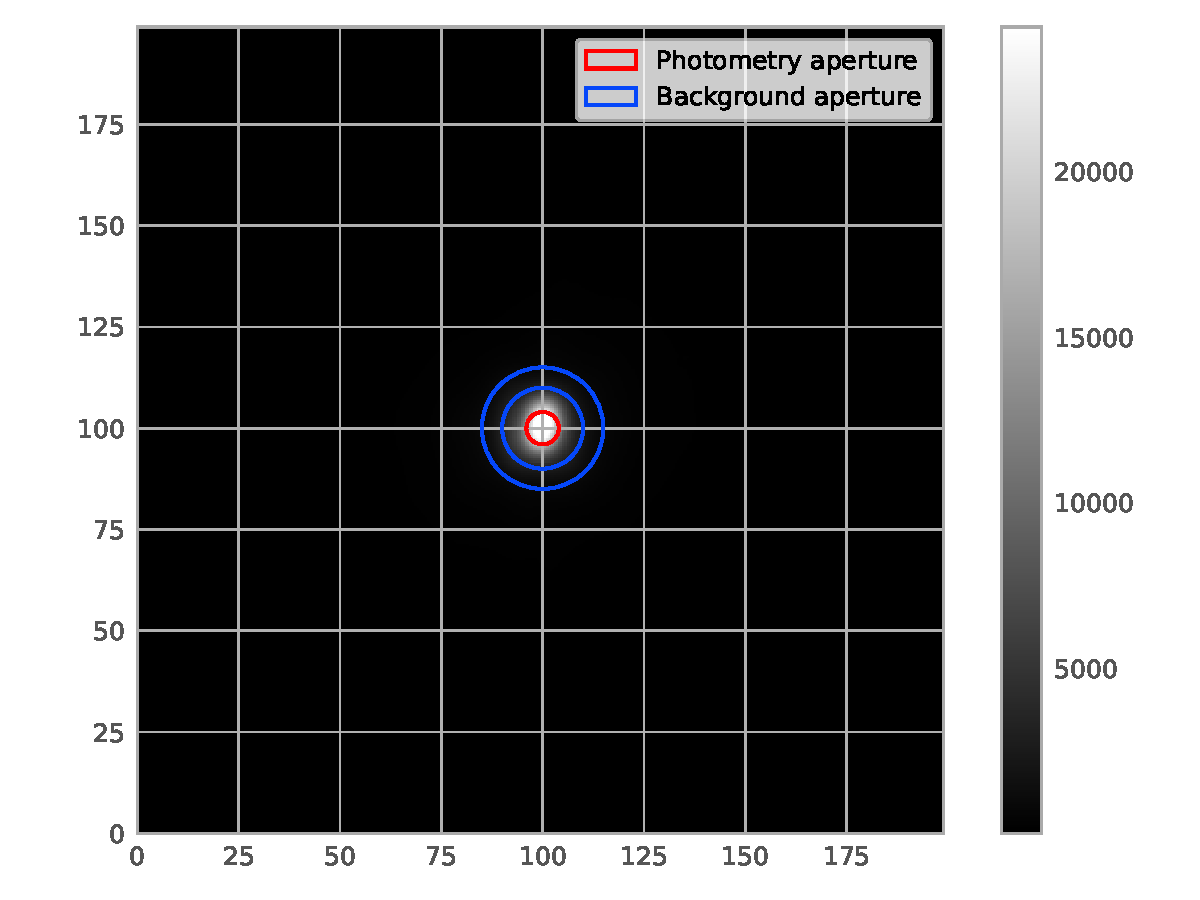
\includegraphics[width=0.9\textwidth]{pics/aperture_example.pdf}
		\caption{An aperture photometry for the star in the center, where the red circle indicates the aperture used and the two blue circles define the annulus used for the background subtraction.}
		\label{fig:aperture_ex}
\end{figure}
From the figure you can see that we chose the annulus not directly after the aperture, but this is just one way to do it. One could also choose the annulus directly after the aperture or choose a different distance between the annulus and the aperture. However the annulus should give a good approximation for the background inside the aperture and therefore it should not be too far away from the aperture. We chose a small distance between the aperture and the annulus of 4 pixels, because we wanted that as little starlight (in this case) as possible is included in the annulus. If we plot the counts per pixels which are included in a certain radius around the star, as it is done in figure \ref{fig:annulus_radi} we see that after around 10 pixels the increase is decreasing rapidly. That is where there is only little starlight left. This is also why we choose the annulus to go from a radius of 10 to 15 pixels. 
\begin{figure}[H]
	\centering
		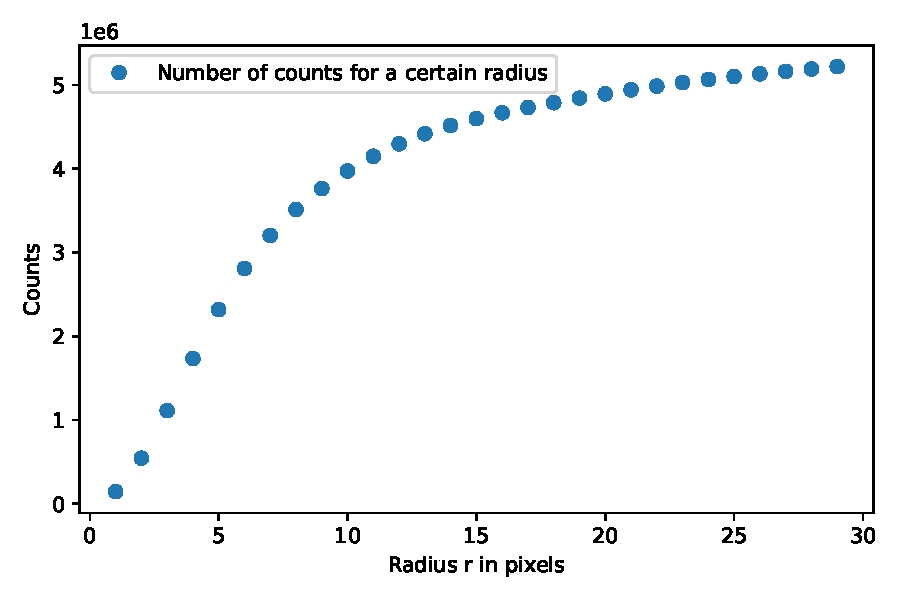
\includegraphics[width=0.8\textwidth]{pics/CountsPerRadius.pdf}
		\caption{The total flux of the star is calculated for different radii and plotted. This shows that after a radius of 10 pixels the contribution from the star is almost gone.}
		\label{fig:annulus_radi}
\end{figure}
Additionally we choose the radius of the aperture to be 6 pixels.

\subsection{Aperture photometry and ghosts}
In order to detect exoplanets one can use aperture photometry. In this subsection we are going to do these steps for the two ghosts which we have in our data from the circumstellar disk HD142527, in order to demonstrate how this could be done for an exoplanet and to learn more about ghosts.\\
A ghost is a copy of the star, which is created by the back-reflection of the star on optical components of the telescope. Figure \ref{fig:ghosts} is an image of HD142527, where the two ghosts are indicated. We see that the ghost on the top right (we will call this ghost 1) is brighter than the ghost on the bottom left (ghost 2). 
\begin{figure}[H]
	\centering
		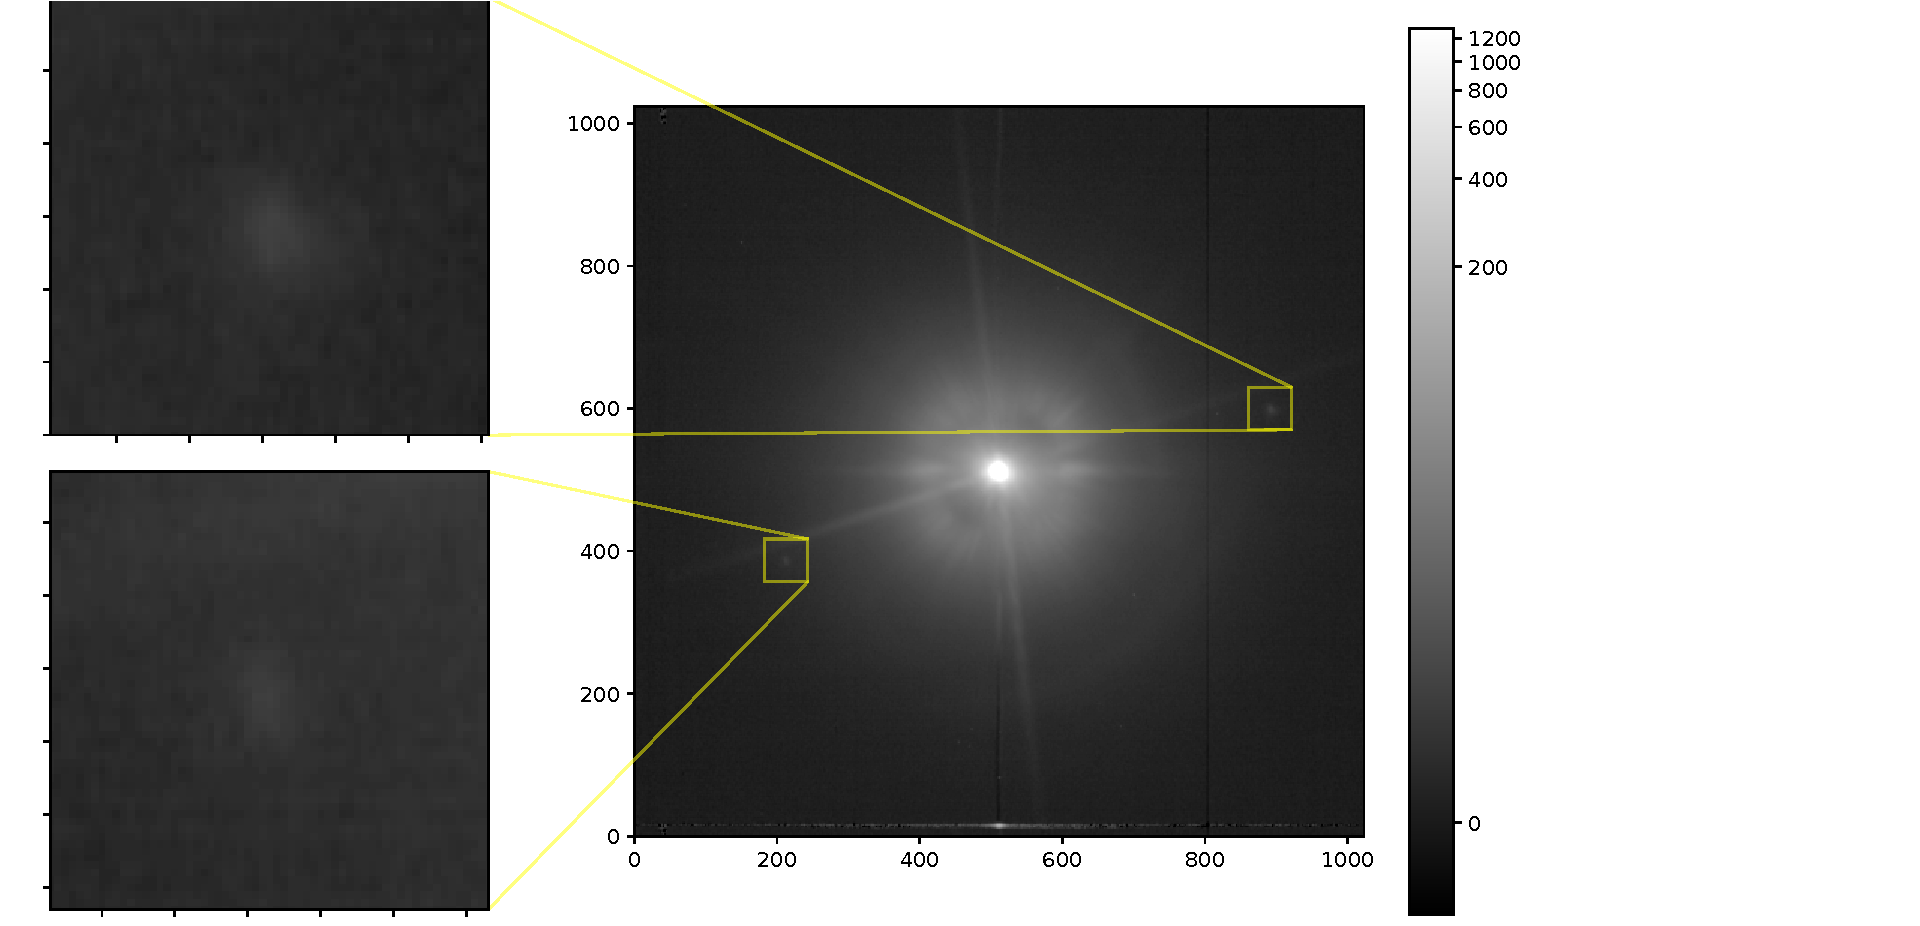
\includegraphics[width=1.3\textwidth]{pics/Ghosts.pdf}
		\caption{An image of the circumstellar disk HD142527, where the two ghosts are indicated.}
		\label{fig:ghosts}
\end{figure}
If we want to confirm the signal from our ghost or also from other objects like exoplanets, which usually can not be seen by eye, we use the signal to noise ratio $S/N$. This means we do aperture photometry for several points around the star which are at the same separation from our star as the ghost (or exoplanet etc.), as in figure \ref{fig:ap_phot_gh1}. From this we can calculate the standard deviation $\sigma$ from the mean of all aperture fluxes and the signal to noise ratio. If the signal to noise ration is larger than the standard deviation, this means that we have a source (ghost, exoplanet) at this position. 
\begin{figure}[H]
	\centering
		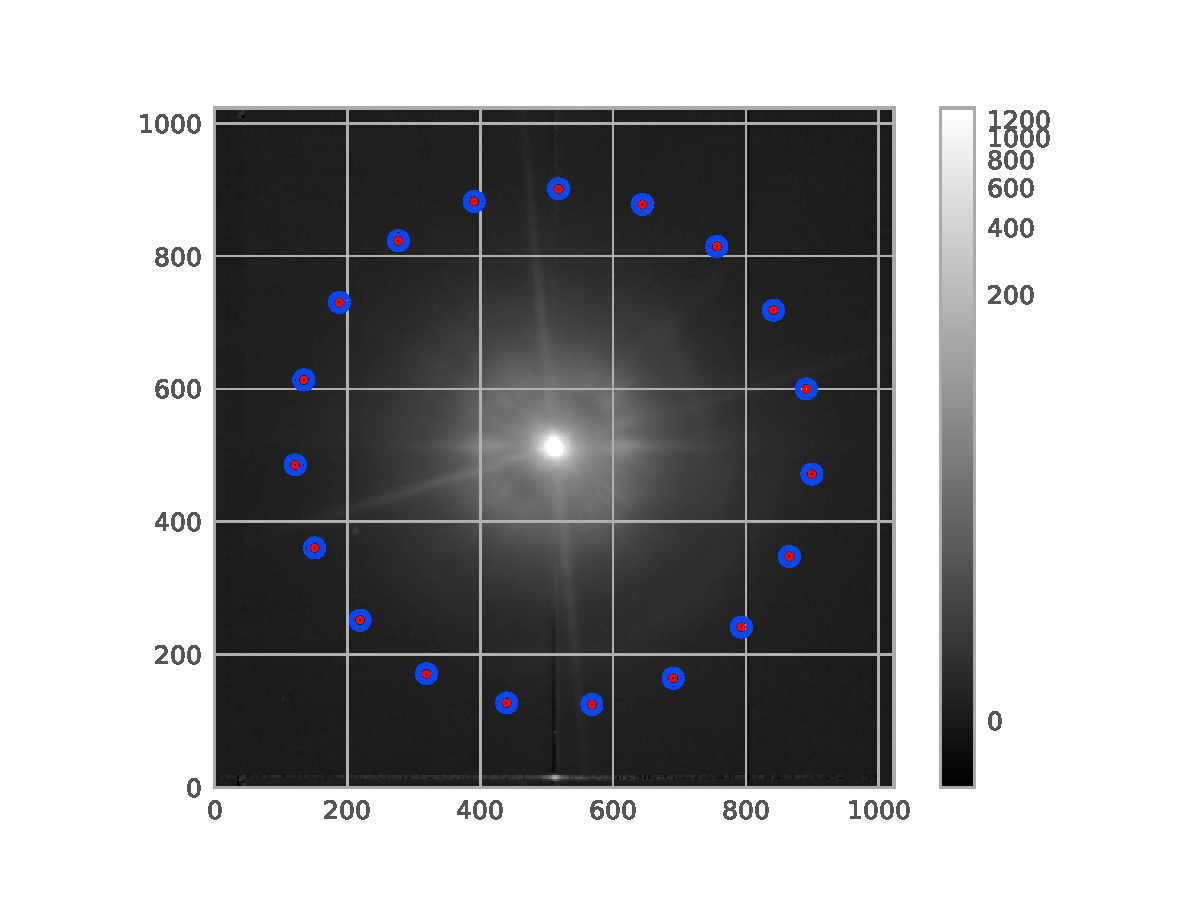
\includegraphics[width=0.9\textwidth]{pics/aperture_photometry_19_ghost1.pdf}
		\caption{In order to confirm the signal from the ghost, we do aperture photometry for several points around the star which are at the same distance from the star as the ghost. We then calculate the standard deviation of all the aperture fluxes and from there find the signal to noise of the ghost's aperture. If the signal to noise is larger than the standard deviation, the position of the ghost is confirmed.}
		\label{fig:ap_phot_gh1}
\end{figure}
The standard deviation is calculated by
\begin{equation}
	\sigma = \sqrt{\frac{1}{k-2} \sum_{ap=2}^{k} (F_{ap} - F_{mean})^2} ,
\end{equation}
where the aperture of the ghost is at $ap=1$, $k$ is the number of apertures and $F_{mean}$ is the mean flux of the apertures (without the aperture of the ghost) given by
\begin{equation}
	F_{mean} = \frac{\sum_{ap=2}^{k} F_{ap}}{k-1} .
\end{equation}
From this we can find the signal to noise ratio as
\begin{equation}
	S/N = \frac{F_1 - F_{mean}}{\sigma} .
\end{equation}
From our data we find a 
\begin{table}[H] 
\label{table:freqtored}
\centering
\caption{The frequency and redshift bins}
\begin{tabular}{|c|c|c|}
\hline
 & Ghost 1 & Ghost 2\\
\hline
$S/N$ & & \\
\hline
\end{tabular}
\end{table}

\section{Transformation to the $r$-$\varphi$ plane}
We have now seen that the ghosts are about $10^{-4}$ times less bright then their star, but potential exoplanets are even less bright. A Jupiter like exoplanet would be $10^{-9}$ less bright (reflecting light) and an Earth like even only $2 \cdot 10^{-10}$. Therefore the data must be really sensitive, with a high contrast and a high spatial resolution. As we can see in figure \ref{fig:ghosts} the star produces strong spiders and speckles which have similar brightness as the ghosts or are even brighter. Therefore exoplanets which are situated in this regimes cannot be detected, unless we are able to take out the signals of the spiders and speckles without taking away other signals, like the ones from exoplanets.\\
If we take a closer look at figure \ref{fig:ghosts} we observe that the structure of the spiders and the speckles are radially oriented around the star. In order to get rid of this effects it might be a good idea to transform the image into the r-phi plane, where we define the star to be at radius zero. After the transformation the spiders and speckles are distributed along the phi axis and they become weaker along the r axis. The image before and after the warping is shown in figure \ref{fig:warping_R150-300}, where we only warped the part of the image which is within radius 150 to 300 pixels. \\
\begin{figure}[H]
	\centering
		\subfigure[]{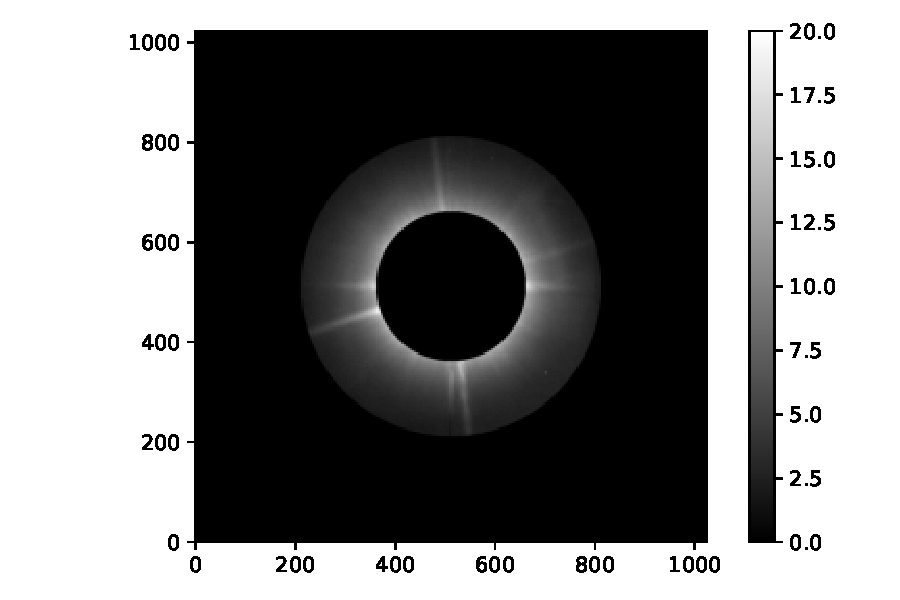
\includegraphics[width=0.6\textwidth]{pics/HDimg_R150_R300.pdf}}
		\subfigure[]{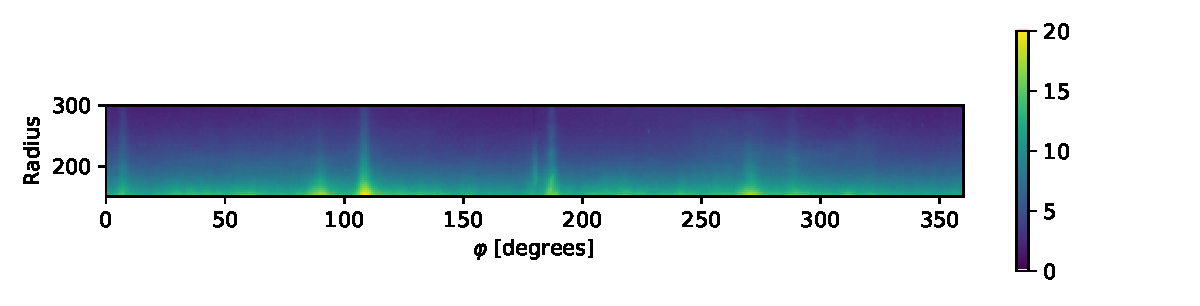
\includegraphics[width=1.1\textwidth]{pics/HDwarped_R150_R300.pdf}}
\caption{We mask the region (radius=150-300 pixels) which will be warped to the $r$-$\varphi$ plane (a). The resulting warped image (b), where we used spline interpolation.}
\label{fig:warping_R150-300}
\end{figure}
Lets have a look at how one can transform the image into the r-phi plane. This kind of transformation is called image warping in image processing. In our case the image warping is based on a specific transformation, namely the transformation from Cartesian to polar coordinates and is therefore also called polar-cartesian distortion.\\
In general an image warping is based on a transformation $T: \mathbb{R}^2 \rightarrow \mathbb{R}^2$, such that 
\begin{equation}
	\vec{x} \mapsto \vec{u} = \begin{pmatrix} T_u(x,y) \\ T_v(x,y) \end{pmatrix},
\end{equation}
where $\vec{x} = \begin{pmatrix} x \\ y \end{pmatrix}$ and $\vec{u} = \begin{pmatrix} u \\ v \end{pmatrix}$. When we want to warp an image $f$ into an image $g$ we do the following calculation
\begin{equation}
	g(\vec{u}) = g(T(\vec{x})) = f(\vec{x}).
\end{equation}
This means that at pixel $\vec{u}$ the computed image $g$ has the same intensity as the original image $f$ at pixel $\vec{x}$. \cite{ImageWarping}\\
When we want to describe the position of a pixel we use Cartesian coordinates, the way it is shown in figure \ref{fig:CoorinateSystems} (a), but there are also other ways to describe the location of the pixels. Figure \ref{fig:CoorinateSystems} (b) shows the image with a polar coordinate system, where we chose the origin to be in the center (where the stars position is).
\begin{figure}[H]
	\centering
		\subfigure[]{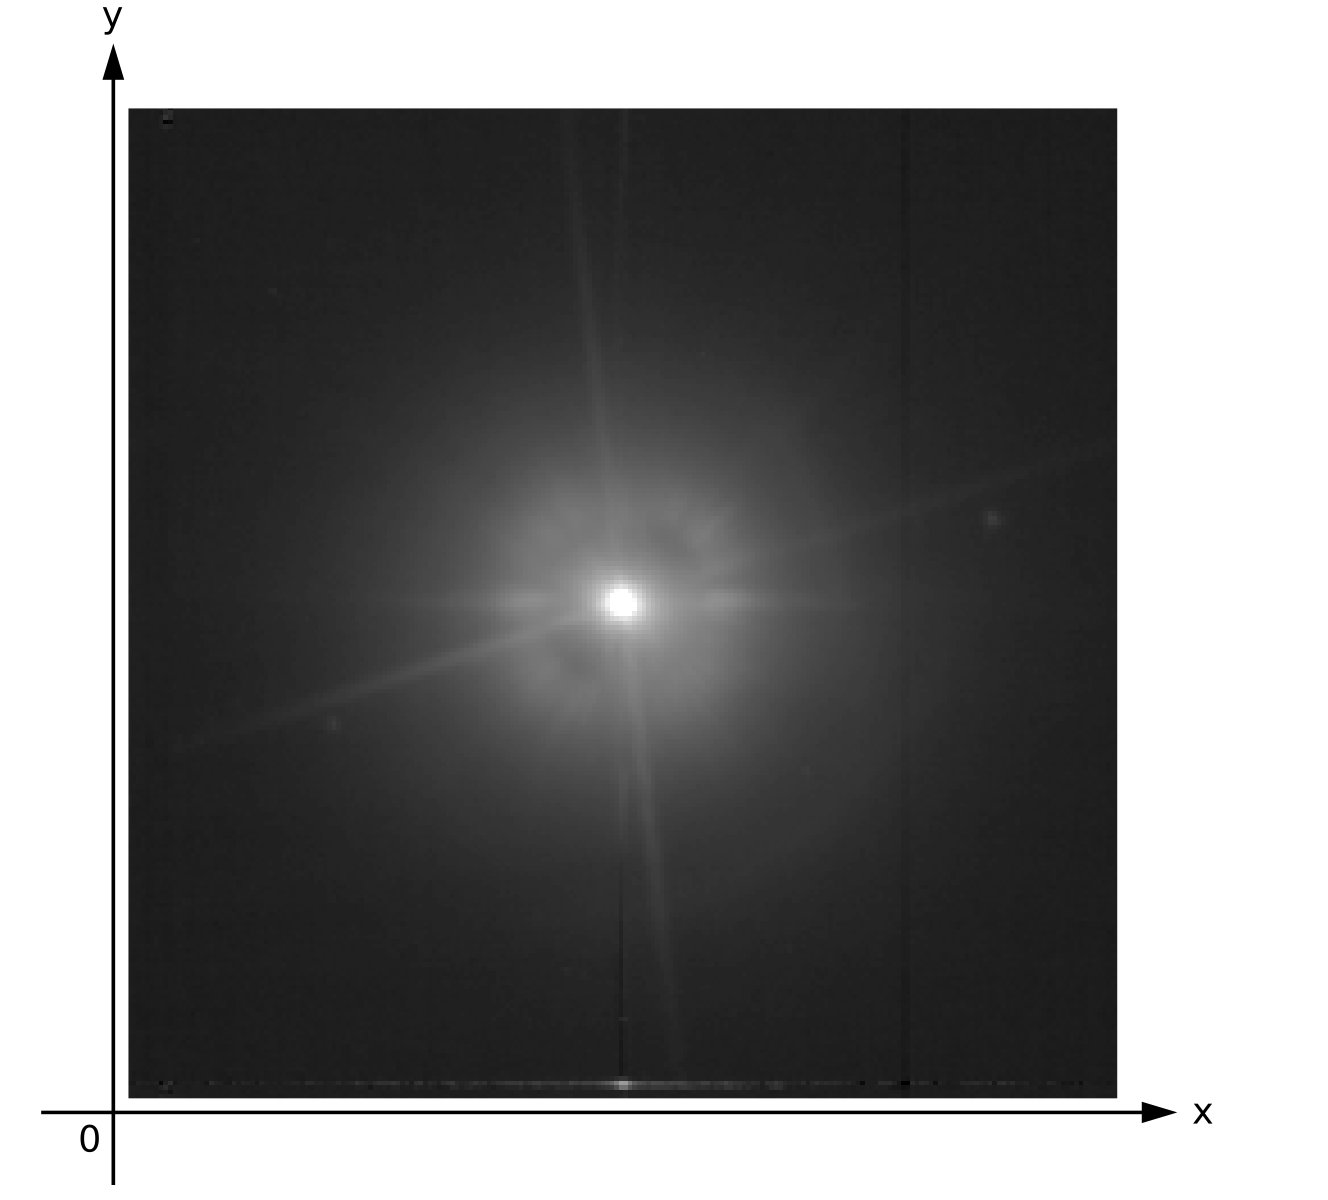
\includegraphics[width=0.49\textwidth]{pics/Star_CartesianCoor.png}}
		\subfigure[]{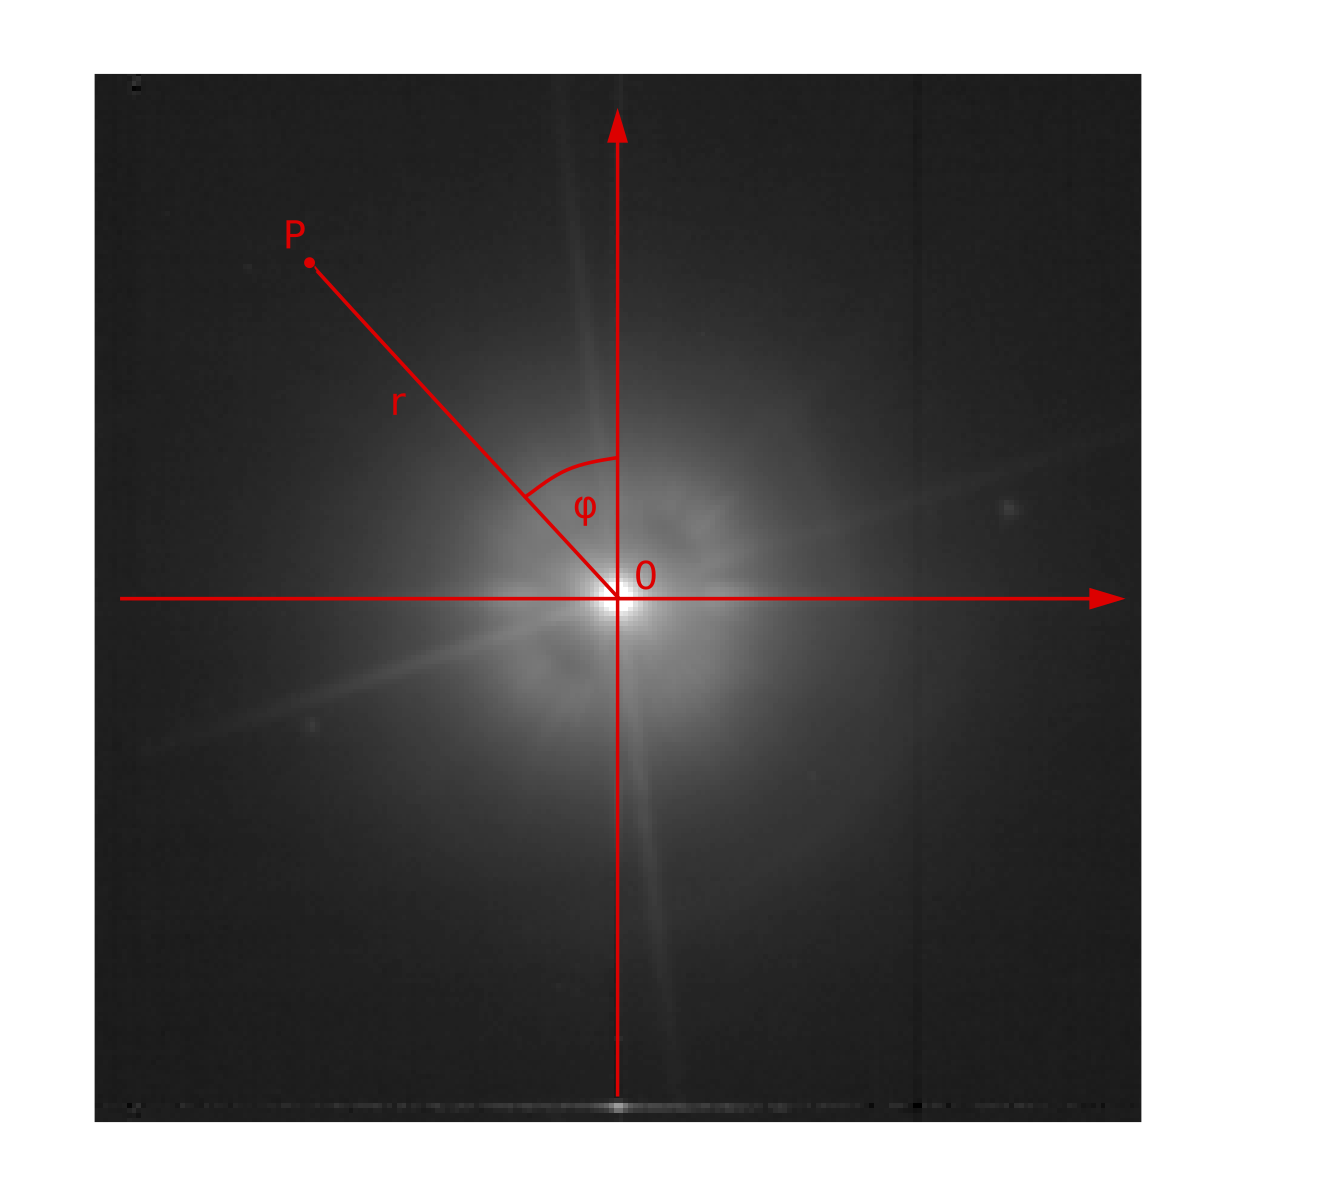
\includegraphics[width=0.49\textwidth]{pics/Star_PolarCoor.png}}
\caption{To describe the location of pixels in an image one usually uses Cartesian coordinates (a), but we can also use polar coordinates (b).}
\label{fig:CoorinateSystems}
\end{figure}
In order to change from Cartesian coordinates $x, y \in \mathbb{R}$ to polar coordinates $r \in [0, \infty)$, $\varphi \in [0, 2\pi)$ one needs to do the following calculations:
\begin{equation}
	r = \sqrt{x^2 + y^2}\\
	\varphi = \arctan \left( \frac{-x}{y} \right).
\end{equation}
For the back transformation from polar to Cartesian coordinates we compute
\begin{equation}
	x = -r \sin(\varphi)\\
	y = r \cos(\varphi).
\end{equation}
The transformation of the pixels from Cartesian to polar coordinates results in pixels which are not squares. However for our resulting image in the $r$-$\varphi$ plane, we need square pixels. This pixel distortion happens because the number of pixels included at a certain radius away from the center increases proportionally to the radius. This means that there are twice as many pixels at a radius of $100$ (pixels) than at radius $50$. We now have two options after we have defined the grid of our $r$-$\varphi$ plane. Either we choose the grid such that at $r=r_{max}$ every pixel in the grid corresponds to a pixel in the original image and for smaller radii we have pixel which are empty. Or we choose the size of the grid differently and use interpolation to assign an appropriate value to each pixel in the $r$-$\varphi$ plane. We decided to use interpolation, since we cannot work with the data if there are empty pixels. In figure \ref{fig:warping_R150-300} we have already seen an example for this transformation using spline interpolation.\\
Now lets think about which length the grid should have. Since our main interest is to find round objects like exoplanets, it would be beneficial if round objects are still round after the transformation. In order for this to be satisfied, the number of pixels at the radius position of the object has to stay unchanged. We therefore decided to choose the radius range (the $\varphi$ angle goes from $0$ to $360$ degrees and thus covers the whole circle), such that the object we want to examine is in the middle and the grid size corresponds to the length of the radius range, i.e. for $r_{min}=100$ and $r_{max}=300$ the length of the grid the radius direction is $r_{len}=r_{min}-r_{max}=200$. The resulting grid size in $\varphi$ direction depends then on the chosen radius range. Namely such that: $\varphi_{len} = 2\pi \cdot (r_{min}+\frac{r_{len}}{2})$.\\
Figure \ref{fig:Circle_distortion} illustrates the effect of this transformation onto circles in the original image (a). In the center of the warped image at $r=200$ the number of pixels is unchanged by the transformation, this means no interpolation nor averaging was needed. Therefore circles stay circles, if they are placed in the middle of the warped image, see figure \ref{fig:Circle_distortion} (c). If we go to larger radii the number of pixels per radius (in original image) increases. Since in the warped image all radii have the same number of pixels $r_{len}$ the transformation averages the information in the original pixels into fewer pixels and the circle becomes elliptic like in its shown in figure \ref{fig:Circle_distortion} (b). The opposite effect happens if we go to smaller radii where the number of pixels per radii (in original image) decreases and interpolation is needed to distribute the original information to an enlarged number of pixels. This results also in an elliptic shape, but with the semi-major axis now in the $\varphi$ direction, see figure \ref{fig:Circle_distortion} (d). 
\begin{figure}[H]
	\centering
		\subfigure[]{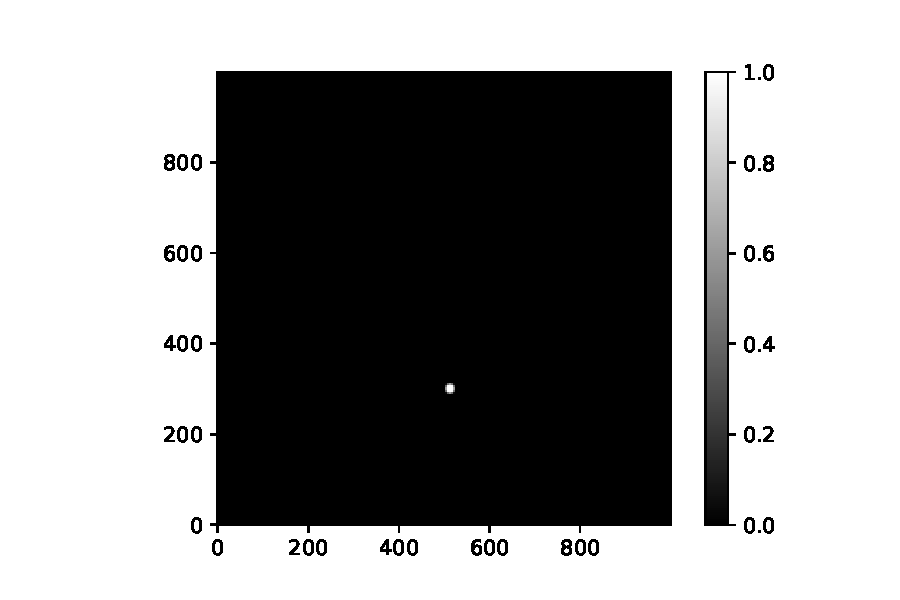
\includegraphics[width=0.6\textwidth]{pics/Circle_image.pdf}}
		\subfigure[]{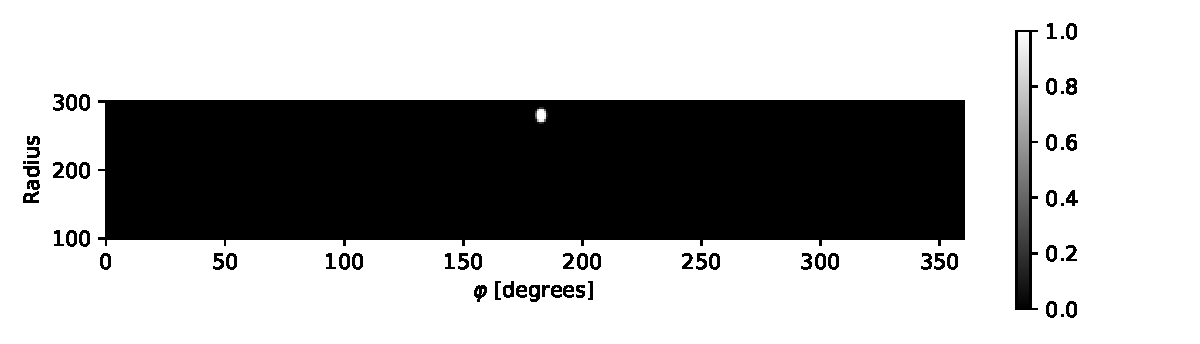
\includegraphics[width=1.1\textwidth]{pics/Circle_top.pdf}}
		\subfigure[]{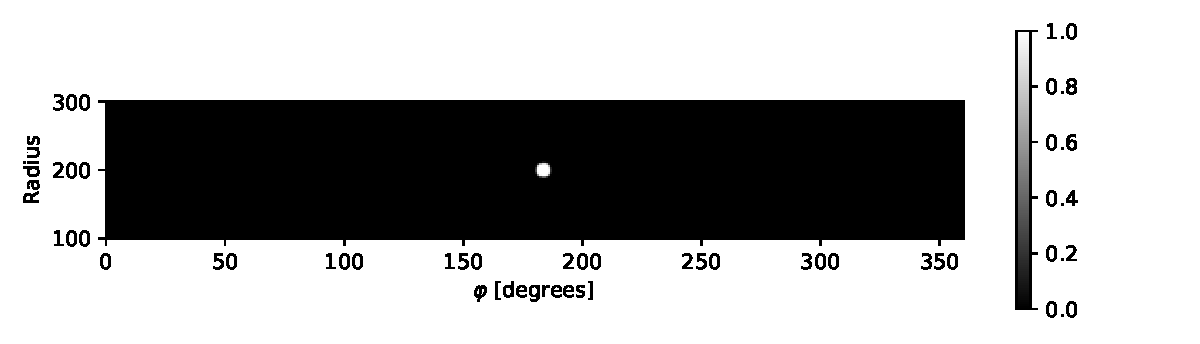
\includegraphics[width=1.1\textwidth]{pics/Circle_center.pdf}}
		\subfigure[]{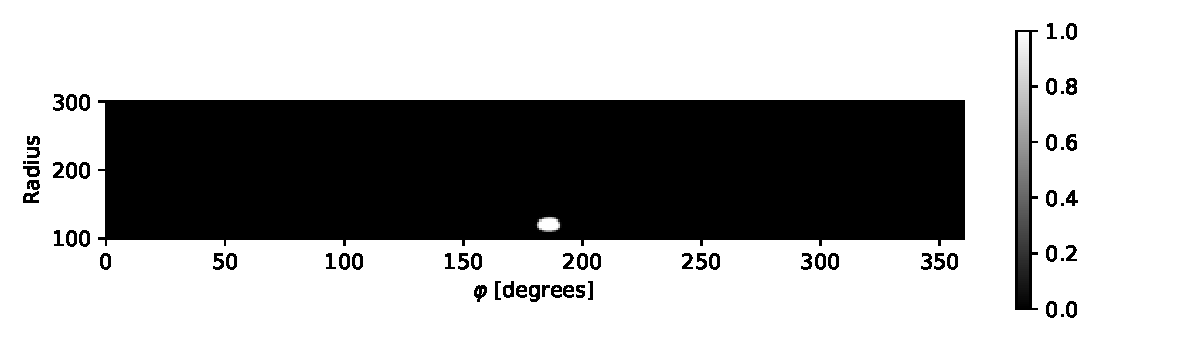
\includegraphics[width=1.1\textwidth]{pics/Circle_bottom.pdf}}
\caption{The warping is defined such that a point in the original image (a) is left unchanged, if it is in the middle of the radius range of the transformed image (c). Otherwise the point will become an ellipse (b) and (d).}
\label{fig:Circle_distortion}
\end{figure}
In order to perform the transformation to the $r$-$\varphi$ plane, we need to define the new shape of the warped image, as discussed before. From this we then define the new pixel grid in polar coordinates and then assign the corresponding Cartesian coordinate values. With this information it is already possible to map the values of the pixels in the original image to the warped one. In our program (shown below \cite{ImageWarping}) we used the python package scipy.ndimage.map\_coordinates() which uses cubic spline interpolation to do the mapping.\\
As we already mentioned interpolation is used to assign a value to every pixel in the new frame by using the information from the old frame. Or in other words the wholes (where we have no information) are closed by cleverly inventing new values for these wholes through the observation of the information in the neighborhood of the whole. The used spline interpolation fits polynomials to the known values (in our case third order polynomials) in the neighborhood and takes then the values given by the polynomials. We chose this method, because we received the best results with it, but one can also use different interpolation methods like nearest neighbor interpolation or the bilinear interpolation. 
\lstset{language=Python, numbers = none}
\begin{lstlisting}[frame=lines]
def to_rphi_plane(image, im_shape, r_min, r_max):
    """
    Warping to r-phi plane.

    Parameters
    ----------
    image : float32, np.array 
        An intensity image.
    im_shape : (int, int)
        Shape of image f.
    r_min : int
        Inner radius.
    r_max : int
        Outer radius.

    Returns
    -------
    warped : float32, np.array 
        r-phi plane image. 

    """
    # Define the shape of the resulting warped image
    r_len = r_max - r_min
    phi_len = int(2*np.pi*(r_min + r_len/2))
    
	# Define the new grid    
    rs, phis = np.meshgrid(np.linspace(r_min, r_max, r_len), 
                           np.linspace(0, 2*np.pi, phi_len), sparse=True)
    
    # Assign the corresponding Cartesian coordinates to the new grid
    xs, ys = rphi_to_xy(rs, phis)
    xs, ys = xs + im_shape[0]/2 -  1, ys + im_shape[1]/2 - 1
    xs, ys = xs.reshape(-1), ys.reshape(-1)
    coords = np.vstack((ys, xs))
    
    # Create the warped image with spline interpolation 3th order
    warped = scipy.ndimage.map_coordinates(image, coords, order=3)
    warped = g.reshape(phi_len, r_len)
    
    return warped
\end{lstlisting}
It is also possible to transform the image back to the Cartesian coordinate map. By simply doing a warping of the image in the $r$-$\varphi$ plane back to the original $x$-$y$ plane.\\
Lets go back to our example with the circle and have a look if the aperture flux of the circle is preserved trough the warping of the image. We find that the circle has an aperture flux of $306$, after the transformation to the $r$-$\varphi$ plane this aperture flux is $302$. So the aperture flux does not change much through the transformation. After the back transformation we get an aperture flux of $306$ which is the same as in the original image. Still we also need to check for this in our data, where we have smooth transitions. We do so by using ghost 1 which is at a radius of $390$ pixels in the data of HD142527. For the flux of the aperture in the image we get $231.5$. After a transformation to the $r$-$\varphi$ plane where we chose $r_{min}=290$ and $r_{max}=490$ the flux of the aperture was $232.1$. This is a change of $0.5 \%$. So we can say that the transformation conserves the aperture flux which is a really good and important property.
\section{Radial intensity drop off}
Due to the star in the center of the image, there is an intensity decrease in radial direction. This light coming from the star makes it harder to find other objects and structures close to it. Therefore we want to get rid it. This is a lot easier in the $r$-$\varphi$ plane, where the intensity decreases is parallel to the $r$ axis as we can see in figure \ref{fig:warping_R150-300} b) and this dropp of can be described by an exponential decrease. In figure \ref{fig:mean_angular_intensity_R150_300} the mean angular intensity values are plotted against the radius and the data is fit by an exponential.
\begin{figure}[H]
	\centering
		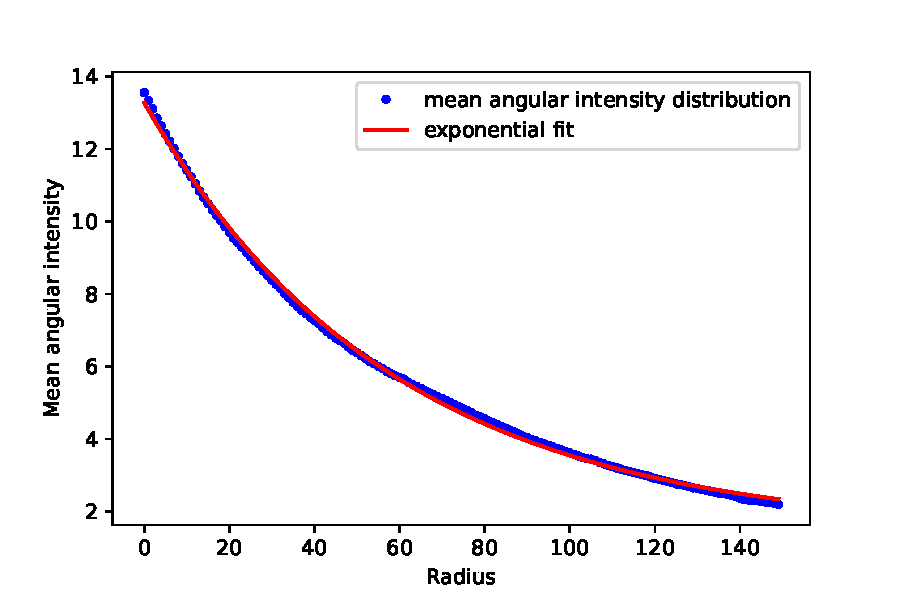
\includegraphics[width=0.9\textwidth]{pics/mean_angular_intensity_R150_300.pdf}
\caption{The intensity drop off due to the light from the star at radius zero can be described by an exponential fit.}
\label{fig:mean_angular_intensity_R150_300}
\end{figure}
The exponential fit describes the intensity drop off in a good way and by subtracting it from the $r$-$\varphi$ plane image we get an image where the mean intensity in radial direction is more or less constant. Figure \ref{fig:flatten_R150-300} shows the effect of this subtraction and we call the resulting image the flatten image.  
\begin{figure}[H]
	\centering
		\subfigure[]{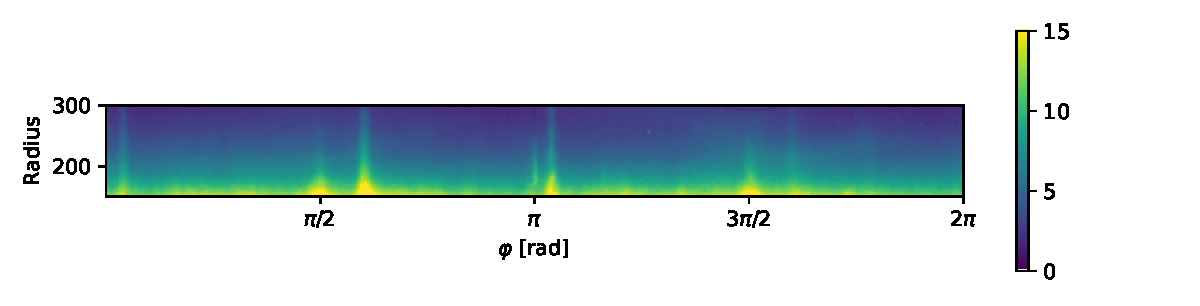
\includegraphics[width=1.0\textwidth]{pics/HDwarped_R150_R300_15.pdf}}
		\subfigure[]{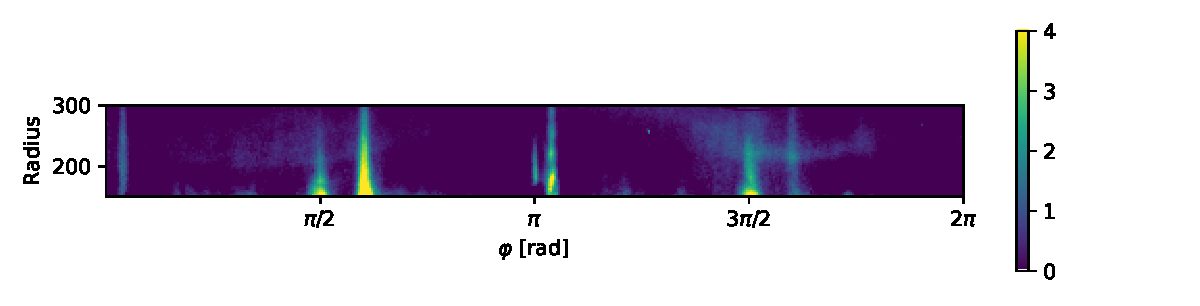
\includegraphics[width=1.0\textwidth]{pics/HDflatten_R150_R300_4.pdf}}
\caption{After the image transformation into the $r$-$\varphi$ plane (a), the image is flattened by subtracting the intensity which comes from the star at radius zero (b).}
\label{fig:flatten_R150-300}
\end{figure}
We insert a model planet (a faint copy of the star) into the image before the flattening of the image to make sure, that the aperture flux is not affected by the flattening. We find that the aperture flux change due to the flattening is only $0.03 \%$. So we can say that the aperture flux is not affected by this procedure. 
\section{Fourier Transformation}
Our goal is to decrease the intensity of the spiders and speckles in the data. In our data from HD142527 the main disturbing effects are the spiders. With the transformation to the $r$-$\varphi$ plane the spiders now are parallel to the $r$-axis. When comparing different data sets from the same observation we find that the spiders change their position, but the distance between them stays the same. It is a periodic pattern. This brings up the question, if the spiders are represented by a set of frequencies in the frequency plane. If this is the case, the suppression of some of the frequencies in the frequency plane would result in a suppression of the spiders in the image plane. The advantage of this method would be that it could be applied to the complete data set and one can ignore the fact that the spiders wander along the $\varphi$-axis. Also we should be able to suppress the spiders without destroying the information below them.\\
For the calculation of the Fast Fourier transform and the inverse Fourier transform we use the numpy package from python as shown in the code fragment below. Since the central frequencies are the most important once, we shift them such that they are in the center of the frequency plane. We also will always plot only the absolute value of the Fourier transforms, unless it is stated differently. 
\lstset{language=Python, numbers = none}
\begin{lstlisting}[frame=lines]
# Calculate the Fast Fourier transform
fourier = np.fft.fftshift(np.fft.fft2(image))

# Transform the Fourier transformed image back to the image plane
image_back = np.fft.ifft2(np.fft.ifftshift(fourier)).real
\end{lstlisting}
In the following we are going to investigate the properties of a Fourier transformation on some specific image structure as lines, beams and point-like sources.\\

\subsection{Lines and Beams}
\label{FFT_Lines_Beams}
We first want to investigate the effect of some simple signals in the image plane on the frequency plane. We choose these signals similar to the shape of the spiders or to the shape of a potential exoplanet, with the goal to identify similar characteristics in the frequency plane of the data.\\
Firstly, we transform a single line (has the width of one pixel) in vertical or horizontal direction to the Fourier plane. A single line in vertical direction ($y$-axis) means that we have a constant signal along the $y$-axis, but we have a non-constant signal in $x$ direction, namely a one pixel wide peak at the $x$ position of the line. So we expect that all $y$-axis frequencies in the Fourier transformed image to be zero, this means that only at $y$ frequency zero we have non-zero values which describe the periodicity in $x$ direction.\\
As we can see from figure \ref{fig:fft_line} the transformation of a single line results into a single line in the frequency plane. The line in the frequency plane is perpendicular to the line in the image plane and is located in the center. This confirms our expectations.\\
Since we plot our results with a logarithmic scale, we need to keep in mind that $\log(0) = -\infty$ . In order to be able to plot our results we added a small value $\epsilon$ to our Fourier transformed results just before plotting.
\begin{figure}[H]
	\centering
		\subfigure[]{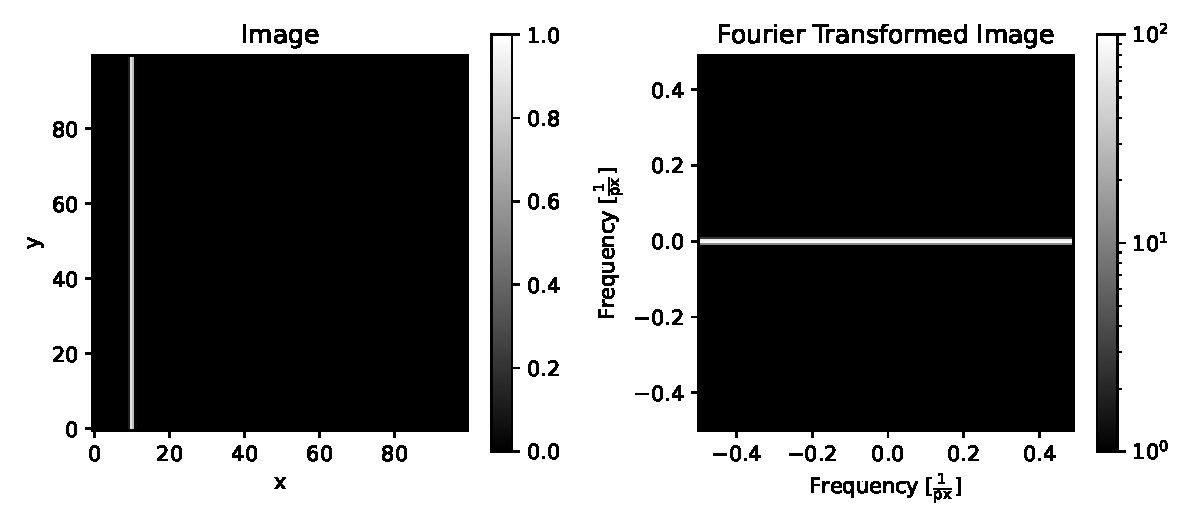
\includegraphics[width=1.0\textwidth]{pics/fft_simulationoneline.pdf}}
		\subfigure[]{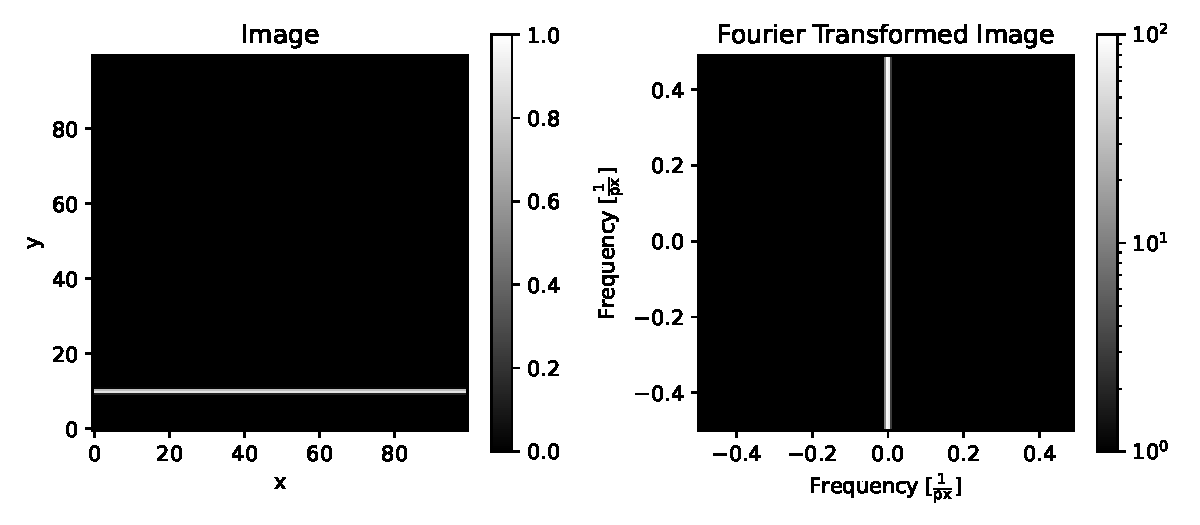
\includegraphics[width=1.0\textwidth]{pics/fft_simulationoneline_horizontal.pdf}}
\caption{The image of a vertical line (a) and of a horizontal line (b) (images on the left side) are transformed to the frequency plane (images on the right side).}
\label{fig:fft_line}
\end{figure}
To explore the frequency plane further we plot the intensity at $y$ frequency equals zero along the $x$ frequency axis (frequency plane of image shown in figure \ref{fig:fft_line} (a)). This describes the periodicity of the image in horizontal direction. As we see in figure \ref{fig:fft_line_cut} the intensity along this axis is constant.
\begin{figure}[H]
	\centering
		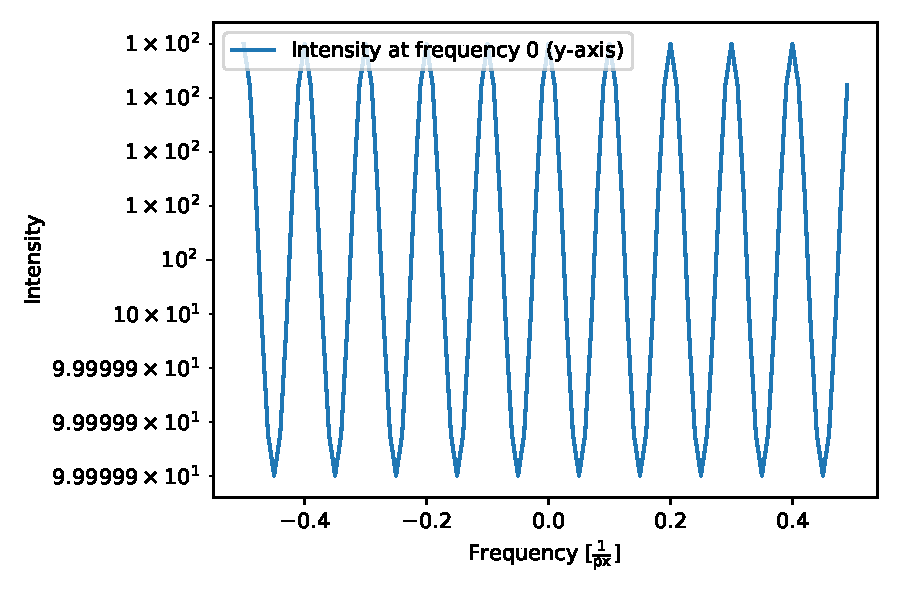
\includegraphics[width=0.8\textwidth]{pics/fft_simulation_cutoneline.pdf}
		\caption{The intensity of the Fourier transformed image in figure \ref{fig:fft_line} (a) at y frequency equals zero.}
		\label{fig:fft_line_cut}
\end{figure}
As a next step we want to find out what happens, if we insert a periodic signal into the image plane in the form of equally spaced lines. Figure \ref{fig:fft_lines} shows an image where there are several vertical lines with a spacing of 20 pixels. As in the case of the single line the image is constant in $y$ direction and so all vertical frequencies are assigned zero. In $x$ direction the lines create a periodic signal with frequency $\frac{1}{20} = 0.05 \frac{1}{\mathrm{px}}$. On the right side of figure \ref{fig:fft_lines} we see the fourier transformation of the image with the equally spaced lines and figure \ref{fig:fft_lines_cut} shows a horizontal cut through the center. We see that only the pixels at $0.05n \frac{1}{\mathrm{px}}$ $\forall n \in \{0, 1, 2, ...\}$ are non-zero.
\begin{figure}[H]
	\centering
		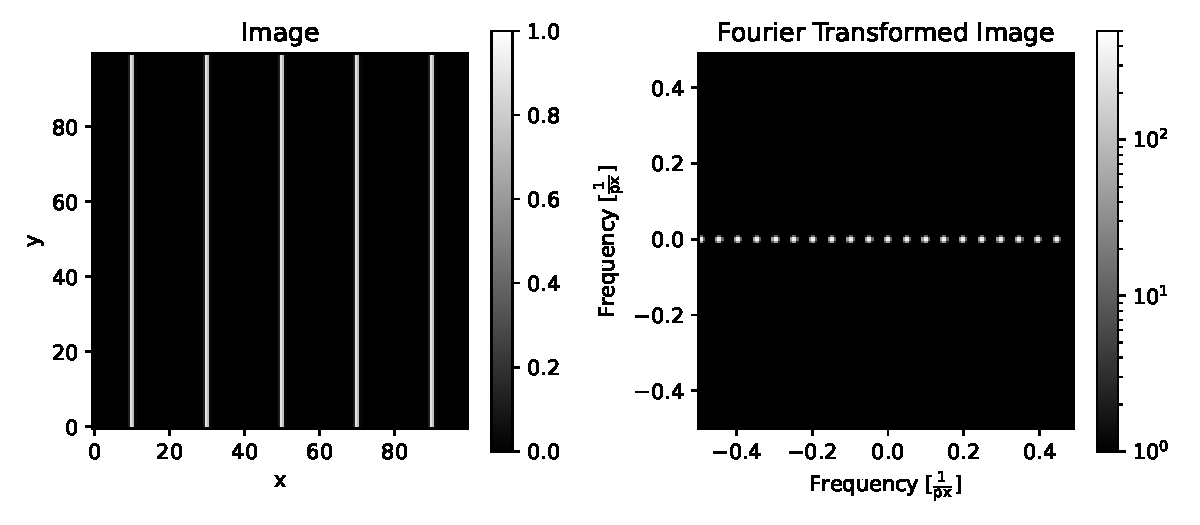
\includegraphics[width=1.0\textwidth]{pics/fft_simulationmorelines.pdf}
		\caption{The image with several equally spaced one pixel thick lines on the left is transformed to the frequency plane, see image on the right.}
		\label{fig:fft_lines}
\end{figure}
\begin{figure}[H]
	\centering
		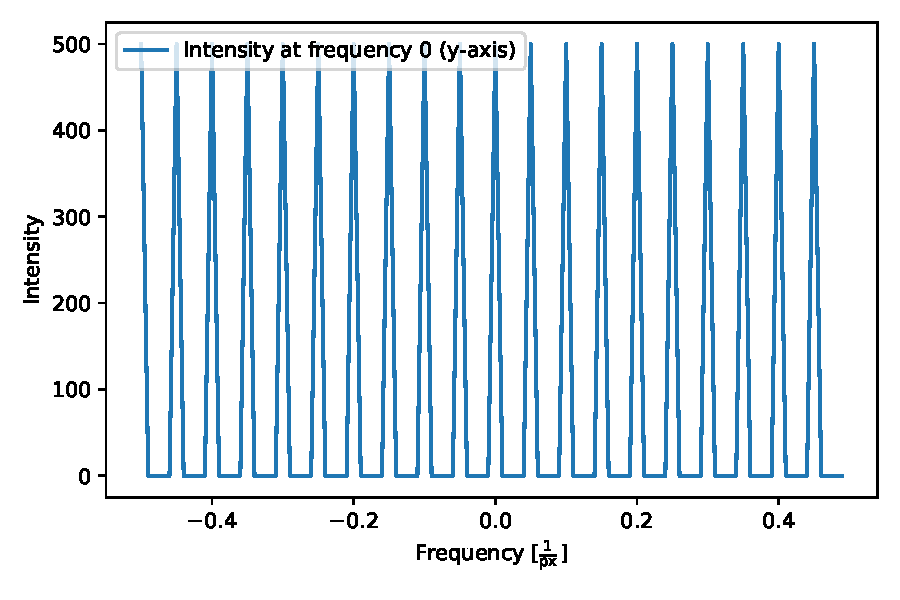
\includegraphics[width=0.8\textwidth]{pics/fft_simulation_cutmorelines.pdf}
		\caption{The intensity of the Fourier transformed image in figure \ref{fig:fft_lines} at y frequency zero.}
		\label{fig:fft_lines_cut}
\end{figure}
In the appendix \ref{almostPeriod} we show, what happens if one line in the periodic image is missing and thus the signal is not completely periodic. We find that the treshold raises up to a higher value.\\
The spiders are not lines, but they have also an expansion into the horizontal, so we are also interested to see the Fourier transform of a single beam. We investigate the image of a beam (stair function) with a width of 10 pixels, placed at $x=10$. Figure \ref{fig:fft_beam} shows the corresponding image and its Fourier transform. As with the lines the only frequencies in the frequency plane with a non-zero value are along the $y=0 \frac{1}{\mathrm{px}}$ frequency axis. Figure \ref{fig:fft_beam_cut} shows this axis in more detail. In contrast to the frequency plane of the line we have a signal which is stronger for central frequencies and decreases slightly for larger frequencies. Additionally we have strong minima at $0.1 n$ $\forall n \in \mathbb{N}$, where the position of the minima is given by one over the width of the beam.
\begin{figure}[H]
	\centering
		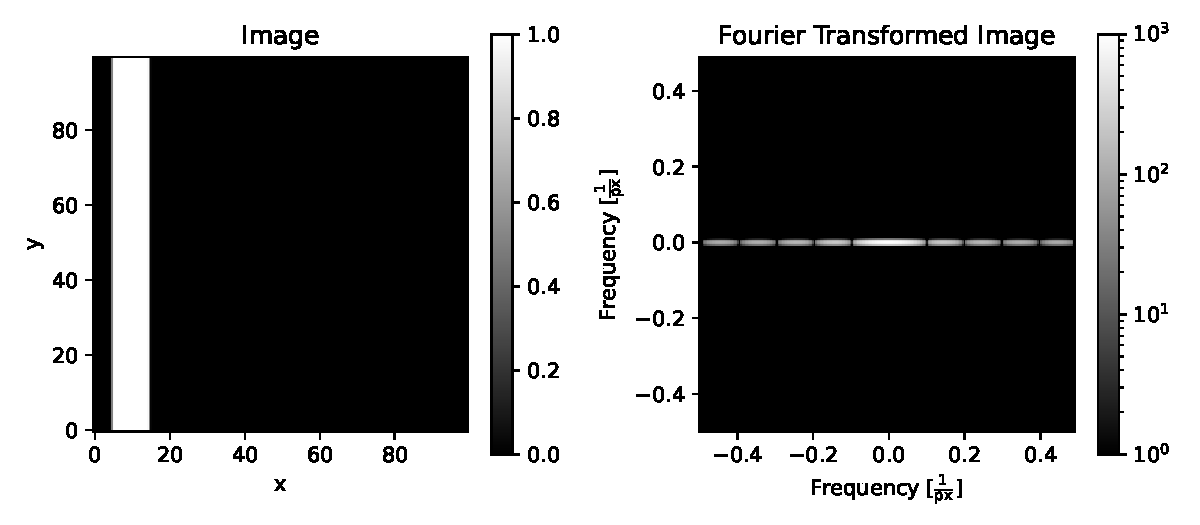
\includegraphics[width=1.0\textwidth]{pics/fft_simulationonebeam.pdf}
		\caption{The image of one 10 pixel thick beam on the left is transformed to the frequency plane, see image on the right.}
		\label{fig:fft_beam}
\end{figure}
\begin{figure}[H]
	\centering
		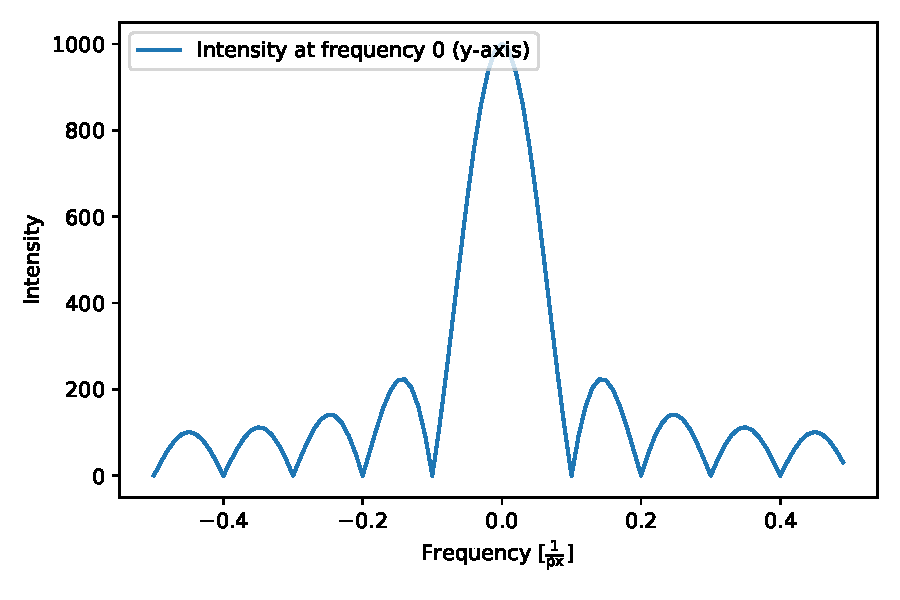
\includegraphics[width=0.8\textwidth]{pics/fft_simulation_cutonebeam.pdf}
		\caption{The intensity of the Fourier transformed image in figure \ref{fig:fft_beam} at y frequency zero.}
		\label{fig:fft_beam_cut}
\end{figure}
As before with the lines we have a look at what happens if we have several of this beams, again equally spaced with a spacing of 20 pixels. We find that this image, lets call it $h(x)$, is a convolution of the image with the equally spaced lines $f(x)$ and the image with the single beam $g(x)$, namely
\begin{equation}
	h(x) = (f * g)(x) = \int_{\mathbb{R}^n} f(\tau)g(x-\tau) \mathrm{d}\tau .
\end{equation}
From the convolution theorem we find that for the Fourier transform it yields:
\begin{equation}
	\mathfrak{F}\{h(x)\} = \mathfrak{F}\{(f * g)(x)\} = (G \cdot F)(\mu),
\end{equation}
where $G(\mu)$ and $F(\mu)$ are the Fourier transforms of $g(x)$ and $f(x)$ \cite{ImageProcessing}. This means that the Fourier transform of the image with the several beams is given by the multiplication of the Fourier transform of the image with the equally spaced lines and the image with the single beam, which can be seen in figure \ref{fig:fft_beams_cut}. Around the center frequency we have some peaks separated by $0.05 \frac{1}{\mathrm{px}} = \frac{1}{20} \frac{1}{\mathrm{px}}$ which describes the separation between the beams of $20$ pixels. This peaks are surrounded by other peaks which are separated by $0.1 \frac{1}{\mathrm{px}} = \frac{1}{10} \frac{1}{\mathrm{px}}$ which describes the width of the beams of $10$ pixels.
\begin{figure}[H]
	\centering
		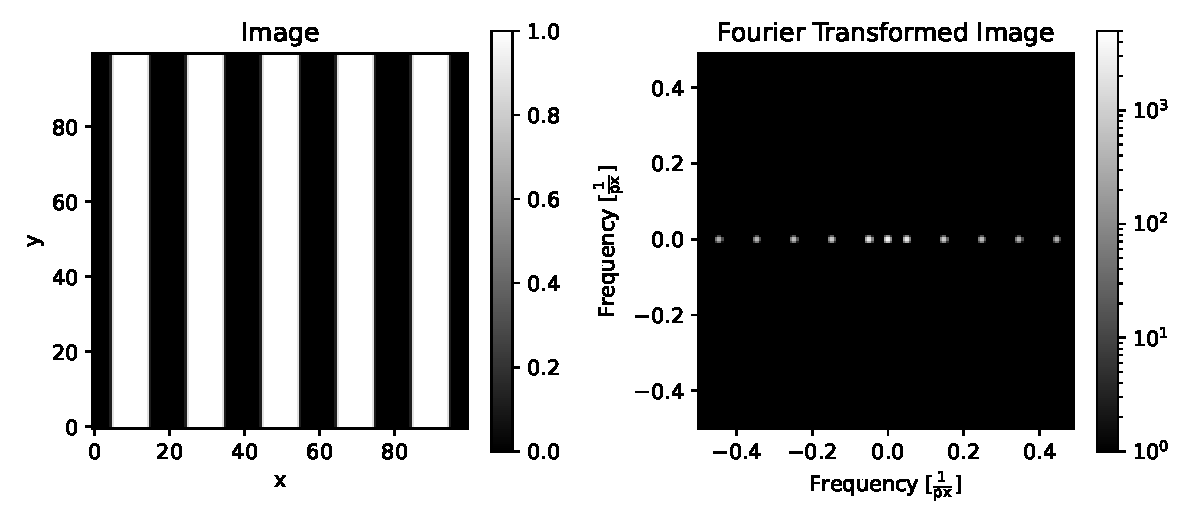
\includegraphics[width=1.0\textwidth]{pics/fft_simulationmorebeams.pdf}
		\caption{The image of several equally spaced 10 pixel thick beam on the left is transformed to the frequency plane, see image on the right.}
		\label{fig:fft_beams}
\end{figure}
\begin{figure}[H]
	\centering
		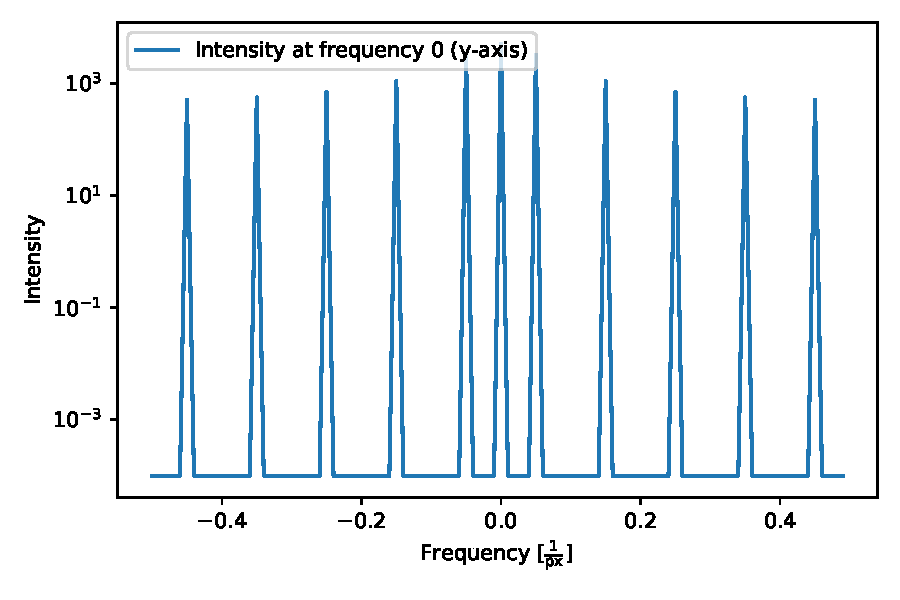
\includegraphics[width=0.8\textwidth]{pics/fft_simulation_cutmorebeams.pdf}
		\caption{The intensity of the Fourier transformed image in figure \ref{fig:fft_beam} at y frequency zero.}
		\label{fig:fft_beams_cut}
\end{figure}

\subsection{Gaussian Beams}
\label{sec:gaussian}
Before we have looked at beams with a stair function shape, but the spiders in our data do not have this stair function shape. In order to have a more realistic approximation we assume the spiders in our simulation to be Gaussian along the radial direction. We calculate the Gaussian profile from 
\begin{equation}
	f(x) = \exp \left(-\frac{(x-\mu)^2}{2 \sigma^2} \right)
\end{equation}
where $\mu$ is the mean (location) and $\sigma$ is the standard deviation (width). \\
Also we change to the image format of the warped image which is not quadratic but rectangular. Four our simulations we choose the radius range 254 to 454 pixels and compare it to the data from HD142527 in this range, which can be seen in figure \ref{fig:warped_254_454}. We have chosen the radius range such that the ghosts lie within it and one of the ghost is in the center of the radius range. So that latter on we can make sure, that we are able to suppress the signal from the spiders without loosing much of the ghosts which we use to simulate a really bright exoplanet. 
\begin{figure}[H]
	\centering
		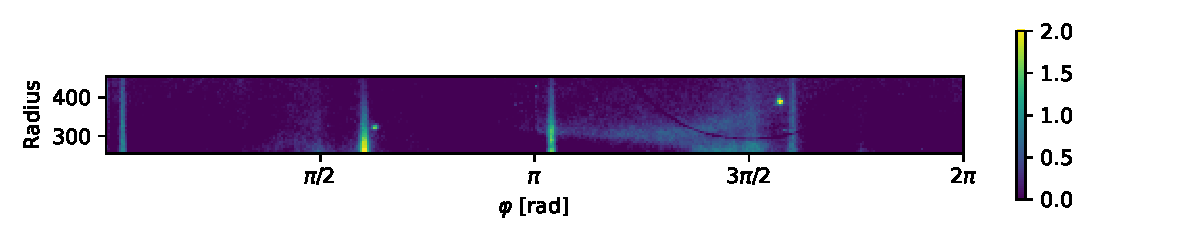
\includegraphics[width=1.0\textwidth]{pics/warped_254_454.pdf}
		\caption{An image of HD142527 which is warped to the $r$-$\varphi$ plane and the radial intensity drop-off is subtracted.}
		\label{fig:warped_254_454}
\end{figure}
Figure \ref{fig:spider_gaussian} shows one of the spiders in a cutout from the image. We can see from the figure that a Gaussian is a good approximation for the shape of the spiders in radial direction.
\begin{figure}[H]
	\centering
		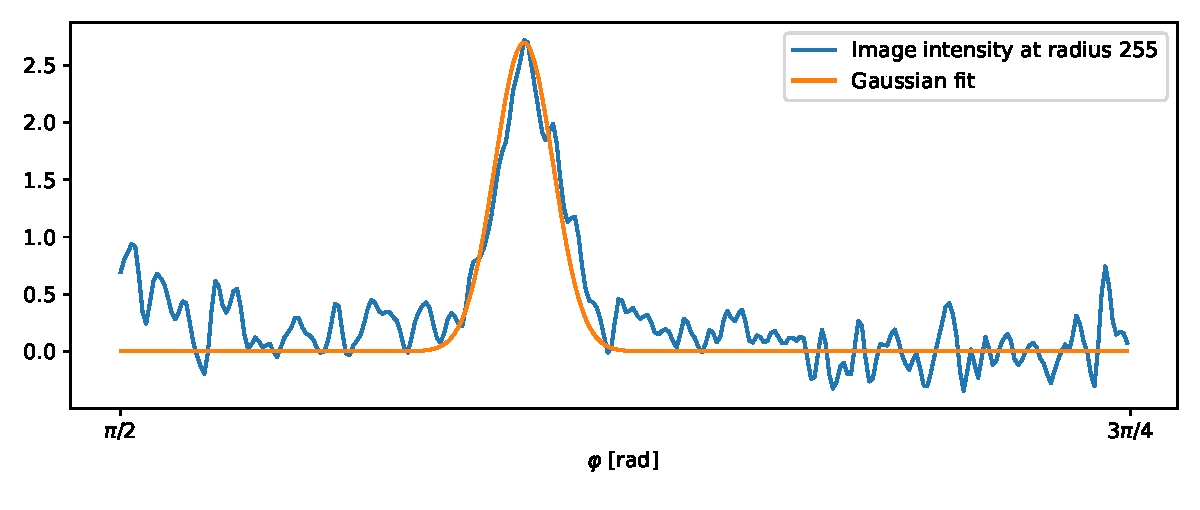
\includegraphics[width=1.0\textwidth]{pics/spyder_gaussian.pdf}
		\caption{A cutout of the image intensity of HD142527 at radius 255, where we see one of the spiders and a Gaussian profile at the same position as the spider is. We can see that the Gaussian is a good approximation for the shape of the spider.}
		\label{fig:spider_gaussian}
\end{figure}
We know that the Fourier transformation of a Gaussian profile is again a Gaussian profile and from the previous subsection we know that the Fourier transform does not depend on the location from the beam, but on the width of it. The spiders in our data all have different widths. In figure \ref{fig:Gauss_diffwidths} we plot four Gaussian profiles with different widths and their Fourier transforms. We see that indeed the Fourier transform of a Gaussian profile is also Gaussian (keep in mind that the plot is logarithmic) and that the width of the Gaussian profile is inverse proportional to the width of its Fourier transform as it already was the case for the stair function beams. Namely that the width of the Fourier transformed Gaussian is $w_{FFT} = \frac{1}{\sigma} \frac{1}{\mathrm{px}}$, where $w_{FFT}$ marks the x-position where the Fourier transformed is again zero. Also the intensity of the Fourier transform decreases with the width of the Gaussian profile, however this effect is rather small in the logarithmic plot. 
\begin{figure}[H]
	\centering
		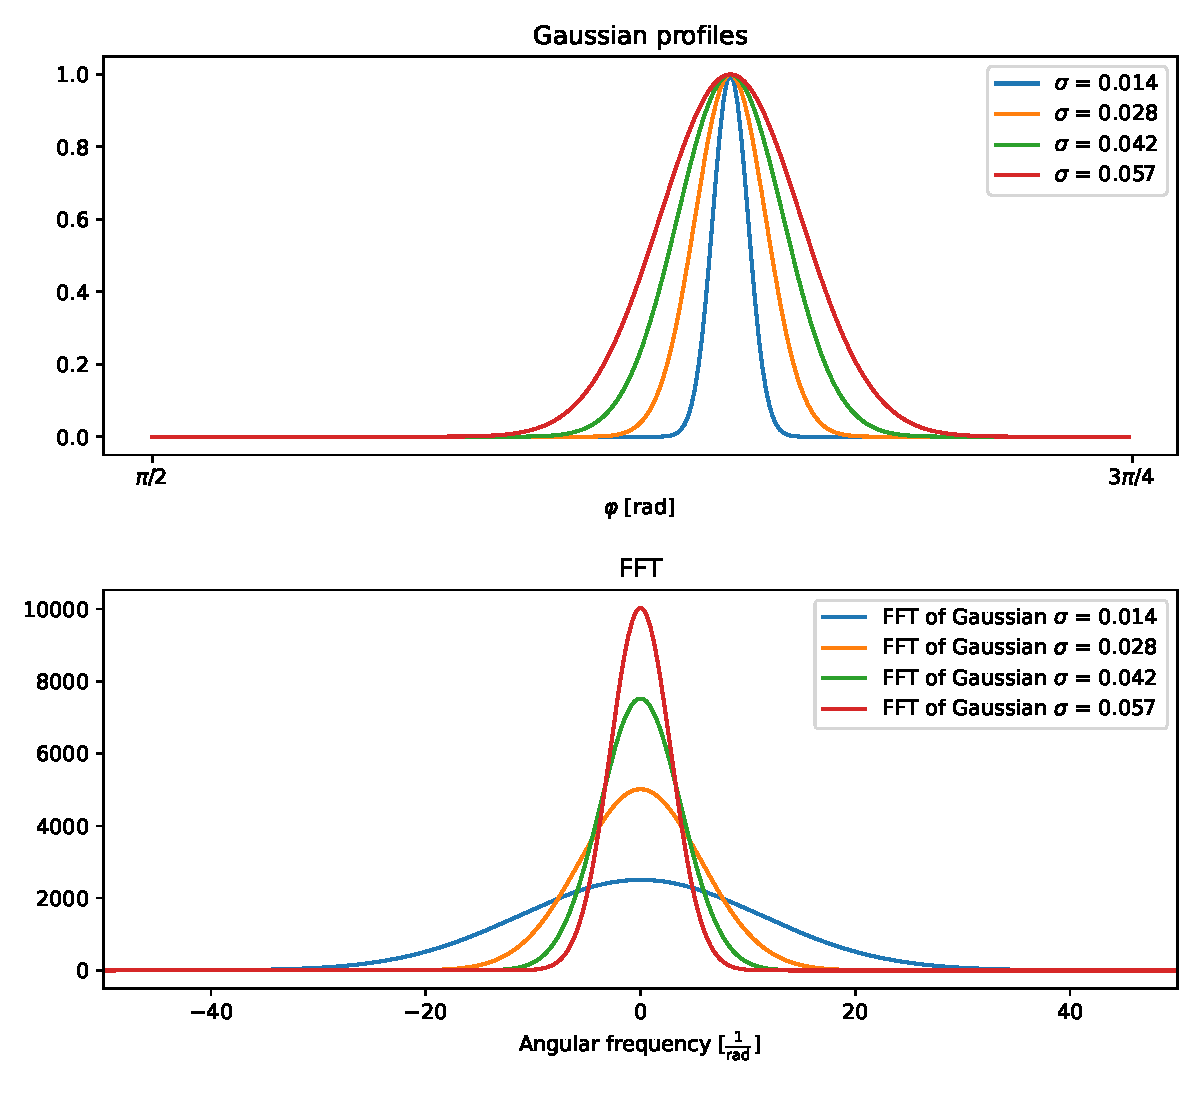
\includegraphics[width=1.0\textwidth]{pics/Gauss_diffwidths.pdf}
		\caption{Gaussian profiles with different widths (top) and the respective Fourier transforms (bottom).}
		\label{fig:Gauss_diffwidths}
\end{figure} 
The VLT telescope produces four spiders which have a 180 degrees symmetry \cite{ESOmanual}. The spiders always have the same distance between each other, but the angular position and width can change from image to image. As a first approximation to this we have a look at four equal Gaussian beams which have the same spacing as in the data and fulfill the 180 degrees symmetry. Figure \ref{fig:Gauss_fourspyders} shows a horizontal cut through this setup and the respective frequency plane. We also plot the Fourier transform of a single Gaussian profile. Due to the linearity of the Fourier transformation we expect the Fourier transformation of the four equal Gaussian to be four times the Fourier transform of the single Gaussian profile. As we see from figure \ref{fig:Gauss_fourspyders}, where also a Fourier transformation of a single Gaussian profile (orange line) is contained, this is also the case, but there is a strong oscillation and a beat as well. To understand this oscillation we can use the knowledge which we have gained when we examined the behavior of the beams with stair function shape. There we found that if the image is a convolution of two different functions, then the Fourier transform is the multiplication of the Fourier transform of each function. \\
For a better understanding we have a look at four Gaussian beams which are all separated by 90 degrees, shown in figure \ref{fig:Gauss_fourspyders90}. Here we have as one function the Gaussian profile with a width of $0.034$ $\mathrm{rad}$,  which if we Fourier transform it produces a Gaussian profile in the frequency plane with a width of $\frac{1}{0.034} = 29.497 \frac{1}{\mathrm{px}}$. The other function in the convolution consists of four lines separated by $\frac{\pi}{2} \mathrm{rad}$, which in the frequency plane corresponds to a large intensity every $\frac{1}{\pi/2} = 0.637 \frac{1}{\mathrm{px}}$ pixel. The multiplication of this two Fourier transformed function results exactly in the image we see in figure \ref{fig:Gauss_fourspyders90}. \\
When we go back to the setting we have in our simulations of the spiders, we do not have equally separated Gaussian profiles. We have the 180 degrees symmetry plus an unknown separation between the neighboring spiders (or Gaussians), this additional information causes an additional convolution which produces the frequency plane we see in figure \ref{fig:Gauss_fourspyders}. 
\begin{figure}[H]
	\centering
		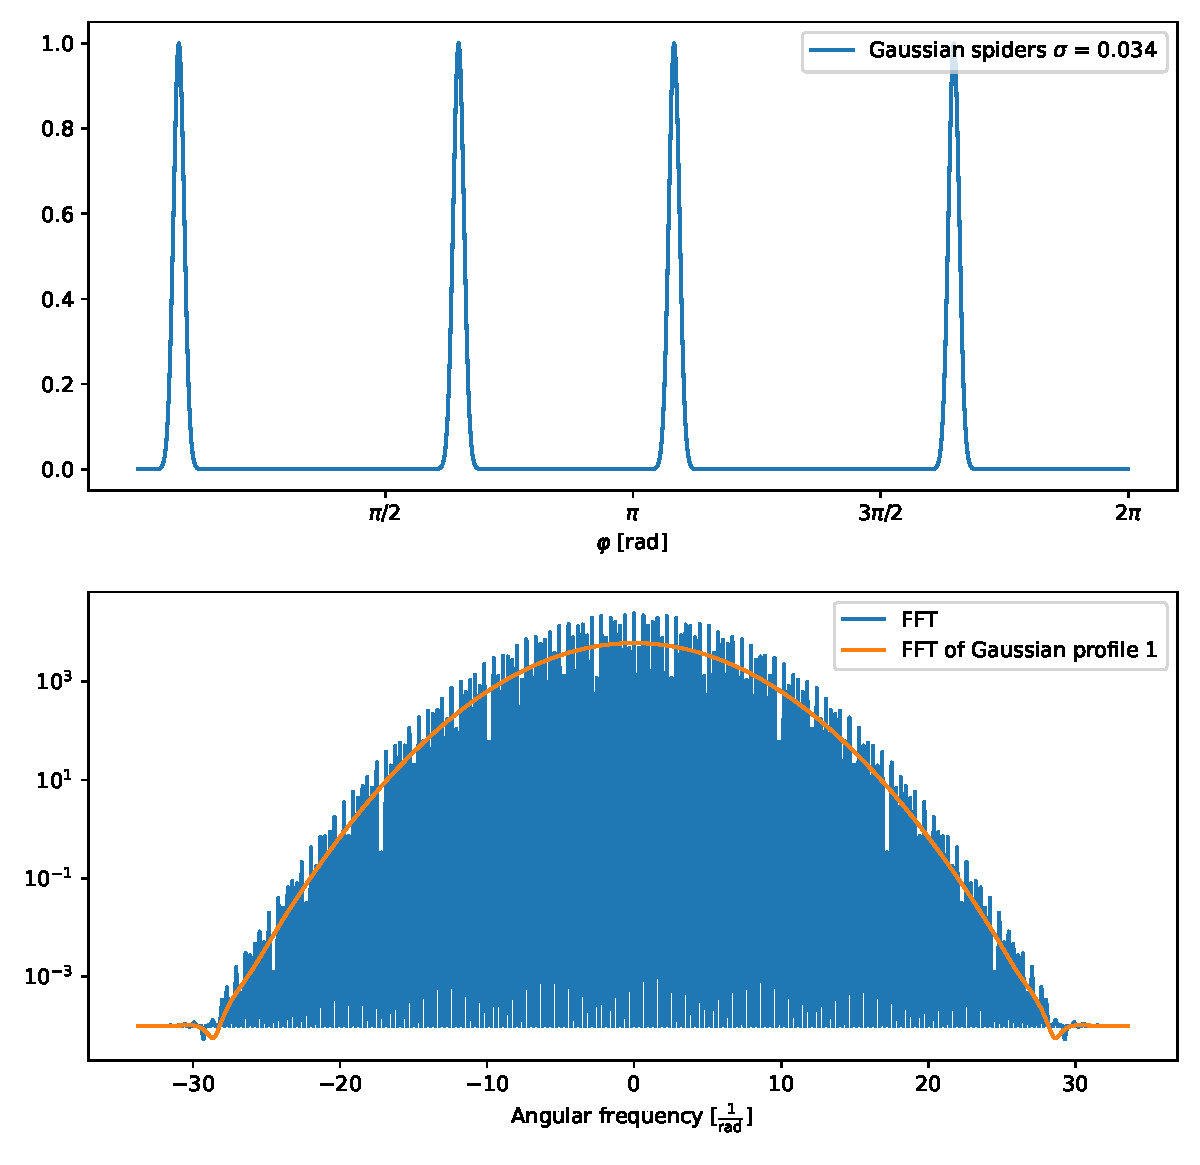
\includegraphics[width=1.0\textwidth]{pics/Gaussian_fourspyders.pdf}
		\caption{The top shows a function with four Gaussian profiles which have a 180 degrees symmetry. The Fourier transform of this is shown in blue in the bottom image. Additionally we plot in orange the Fourier transform of a single Gaussian profile.}
		\label{fig:Gauss_fourspyders}
\end{figure} 
\begin{figure}[H]
	\centering
		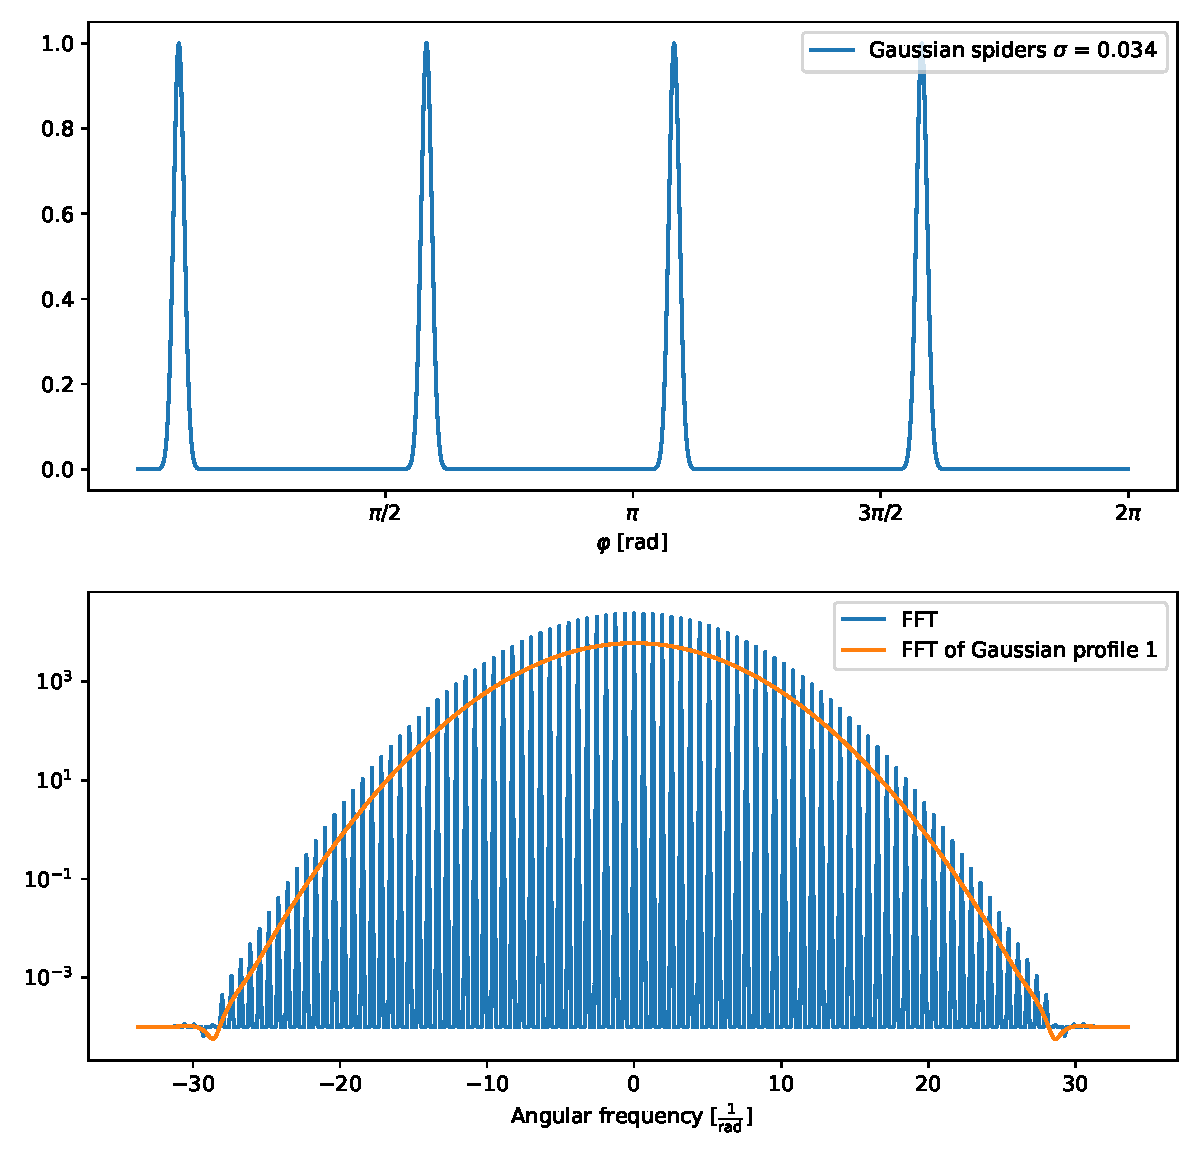
\includegraphics[width=1.0\textwidth]{pics/Gaussian_fourspyders90.pdf}
		\caption{The top shows a function with four Gaussian profiles every 90 degrees. The Fourier transform of this is shown in blue in the bottom image. Additionally we plot in orange the Fourier transform of a single Gaussian profile.}
		\label{fig:Gauss_fourspyders90}
\end{figure} 
As a next step we want to include the fact, that the spiders have different widths, see figure \ref{fig:Gaussian_fourdiffspyders}. As we saw from figure \ref{fig:Gauss_diffwidths} the width of the Gaussian mainly influences the width of the Fourier transformed Gaussian and its height. As before we can use the linearity of the Fourier transformation, but now we add up four different Gaussian profiles. Therefore the resulting Fourier transform has the width of the Fourier transform of the thinnest Gaussian profile and the height of the Fourier Transform from the thickest Gaussian profile. We see that the oscillation caused by the convolutions only starts to play a role when the intensity from the respective profile is large enough. 
\begin{figure}[H]
	\centering
		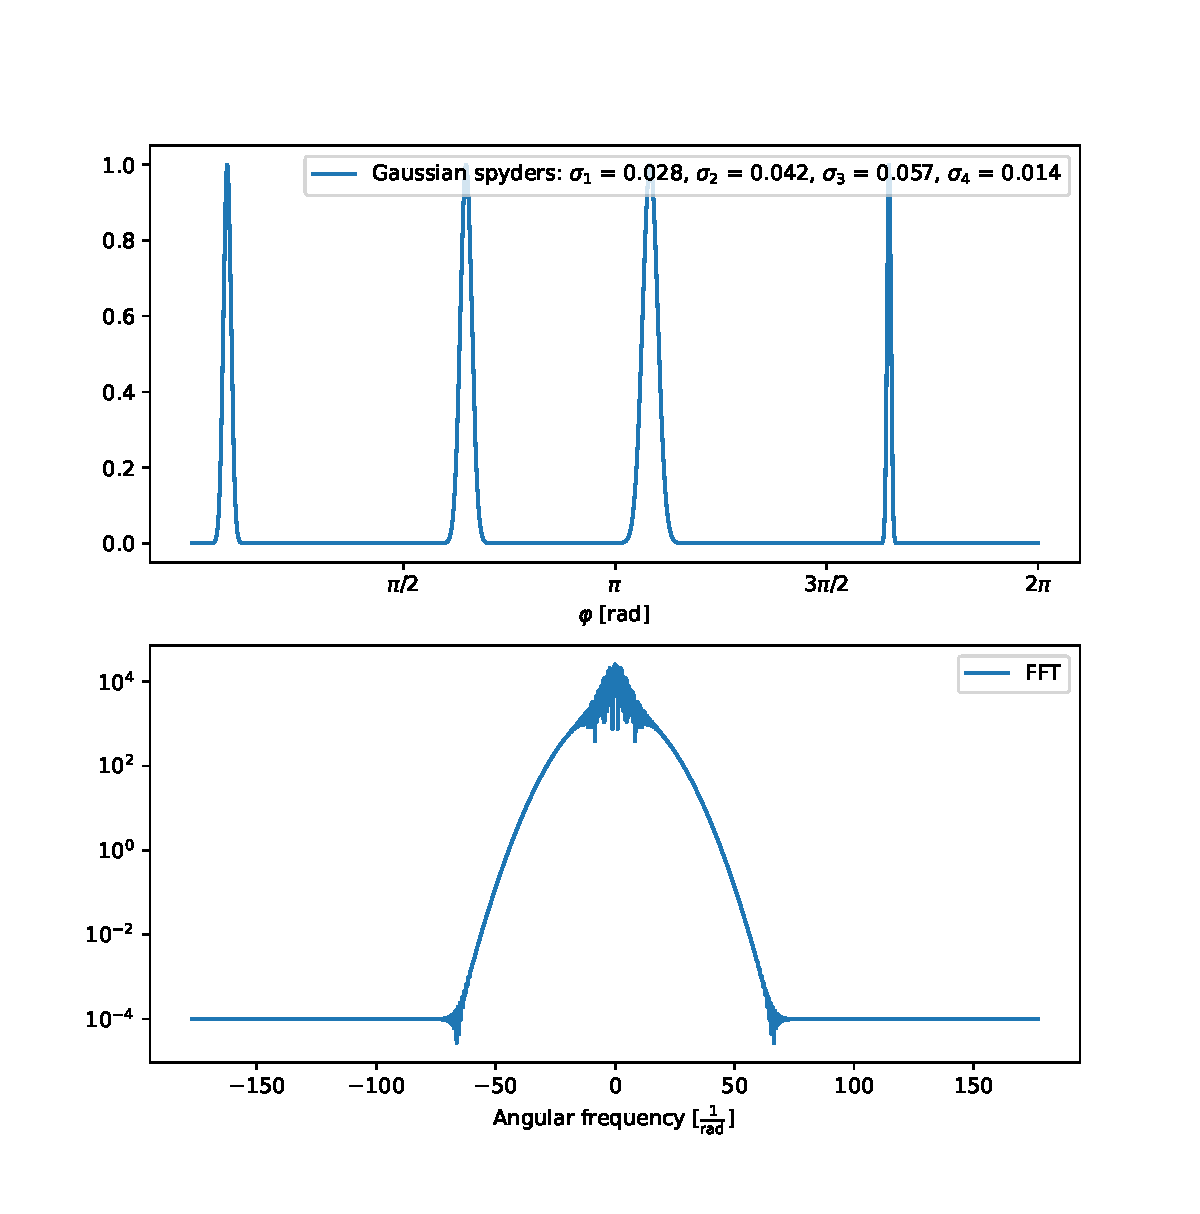
\includegraphics[width=1.0\textwidth]{pics/Gaussian_fourdiffspyders.pdf}
		\caption{The top shows a function with four Gaussian profiles of different widths which have a 180 degrees symmetry. The Fourier transform of this is shown in the bottom image.}
		\label{fig:Gaussian_fourdiffspyders}
\end{figure} 
Finally we also need to take into account that the spiders have different intensities/heights. We look again at the four Gaussian profiles with equal widths which have a 180 degrees symmetry. This time the four Gaussian profiles have different heights as it is shown in the image at the top of figure \ref{fig:Gaussian_fourheightspyders}. Figure \ref{fig:Gaussian_fourheightspyders} also shows the Fourier transform of each profile. We see that the Fourier transform of a profile with a higher intensity also has a higher intensity. When we Fourier transform the whole function which contains all four Gaussian profiles, we get the same Fourier transform as for the one with four equal Gaussian profiles, see figure \ref{fig:Gauss_fourspyders}, but the intensity of the oscillations is smaller and the intensity of the Fourier transform is the summation of the Fourier transform of each profile. 
\begin{figure}[H]
	\centering
		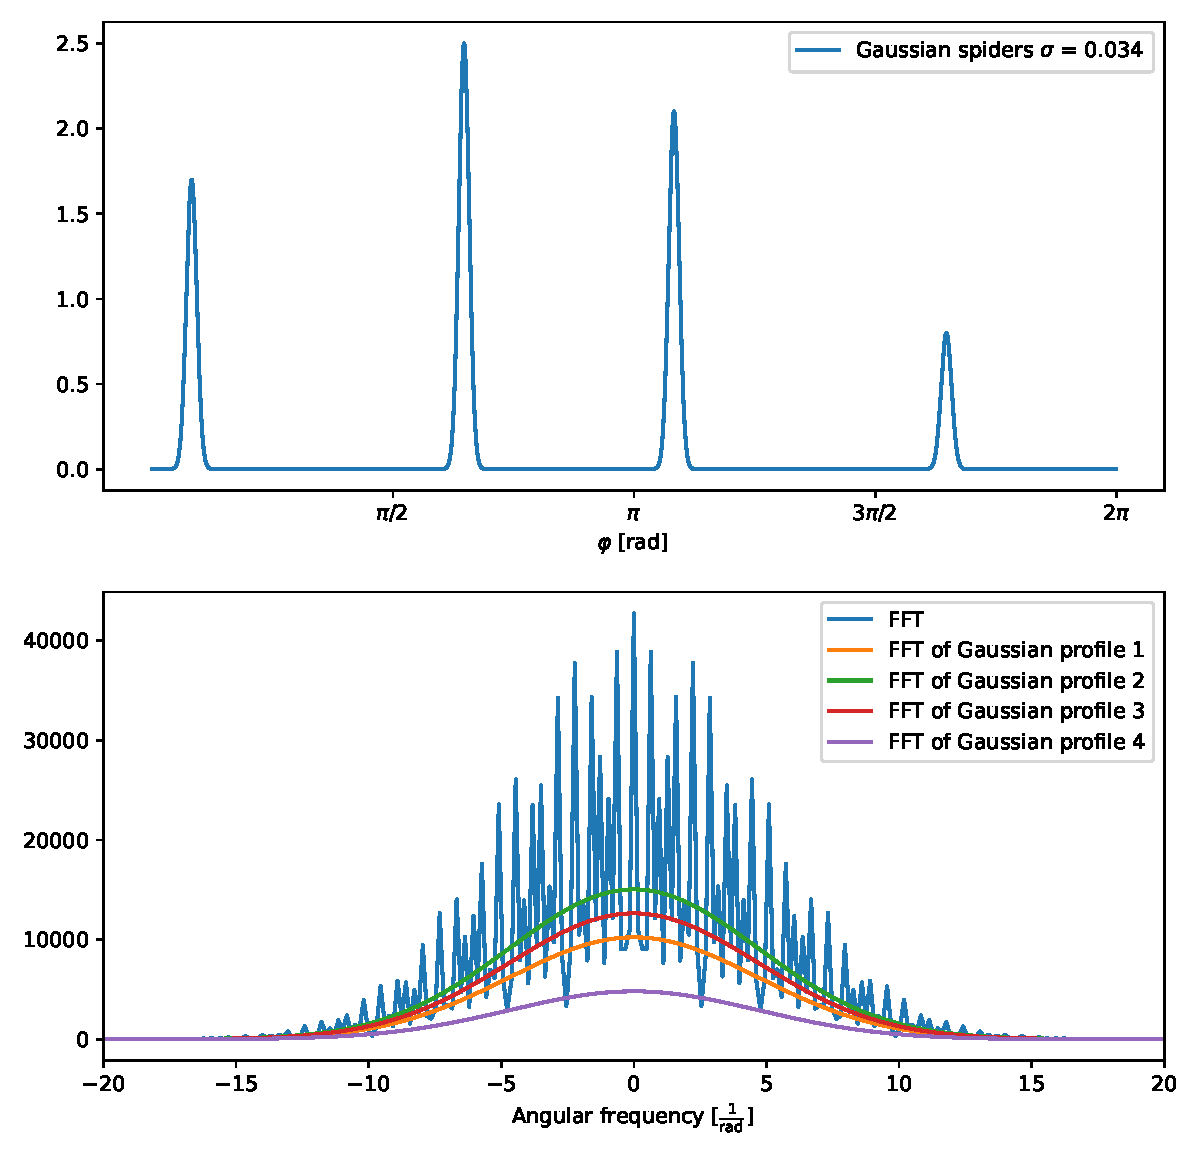
\includegraphics[width=1.0\textwidth]{pics/Gaussian_fourheightspyders.pdf}
		\caption{The top shows a function with four Gaussian profiles of different heights which have a 180 degrees symmetry. The Fourier transform of this is shown in the bottom image.}
		\label{fig:Gaussian_fourheightspyders}
\end{figure}
In conclusion we can say that for four spiders with a 180 degrees symmetry which have different widths and different heights the important frequencies are around the center frequencies. Also the strength of the oscillations are due to the different widths and heights not really strong, so that the intensity could also be approximated by the mean value to cancel out the oscillations.  

\subsection{Spiders}
For the simulation of the spiders we use the knowledge which we have gained before from the Gaussian beams. In angular direction the spiders have a profile which is similar to a Gaussian, we therefore use Gaussian profiles for the simulation. In radial direction the spiders get thinner and their intensity decreases. Additionally all spiders have different widths and heights/intensities. Figure \ref{fig:simulated_spyder} shows the simulation of the spiders and the Fourier transformation of it. We see that in contrast to the Fourier transformation of the beams, Gaussian or stair function, there are not only non-zero frequencies at radial frequency zero, but they spread into all radial frequencies around the central angular frequencies. This radial spread is caused by the change of the width and intensity in radial direction.\\
\begin{figure}[H]
	\centering
		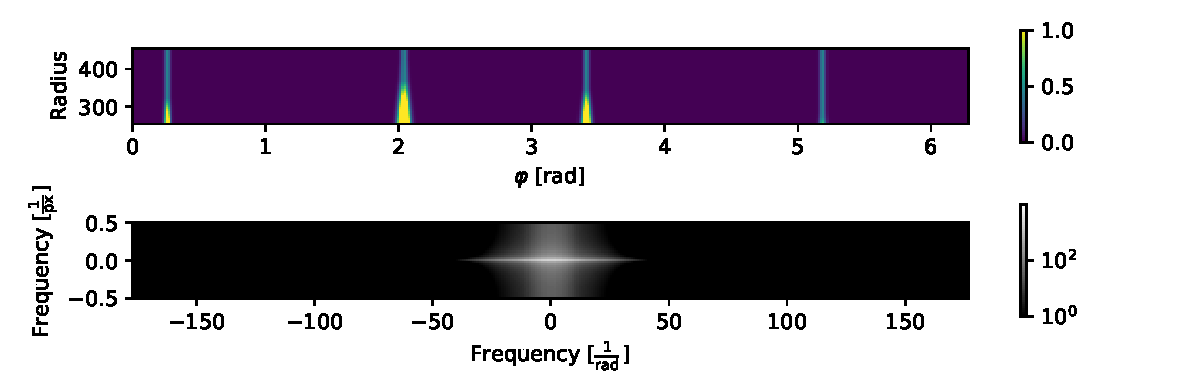
\includegraphics[width=1.0\textwidth]{pics/simulated_spyder.pdf}
		\caption{For a better understanding we simulate the spiders (top) and Fourier transform it (bottom).}
		\label{fig:simulated_spyder}
\end{figure}
For a better understanding of the Fourier transformation, we plot the Fourier transform at different radial and angular frequencies, see figure \ref{fig:simspi_angularfreq} and \ref{fig:simspi_radialfreq}.\\
We find that the intensities at radial frequency zero are the same as if the spiders would be Gaussian beams, with the intensity and widths being constant in radial direction. This means the width is defined by the inverse of the width of the smallest spider and the shape around the peak is dominated by the Fourier transform of the thickest spider. The maximal intensity is a sum of all Fourier transformed Gaussian profiles and the oscillations are due to the distances between the spiders. \\
For radial frequencies other than zero the intensity decreases rapidly to a small value and then stays constant, see figure \ref{fig:simspi_radialfreq}. This can also be seen in figure \ref{fig:simspi_angularfreq}, and therefore the important frequencies are for radial frequencies larger/smaller than approximately $-0.06$/$0.06$ $\frac{1}{\mathrm{px}}$ and for angular frequencies larger/smaller than approximately $-30$/$30$ $\frac{1}{\mathrm{rad}}$.
\begin{figure}[H]
	\centering
		\subfigure[]{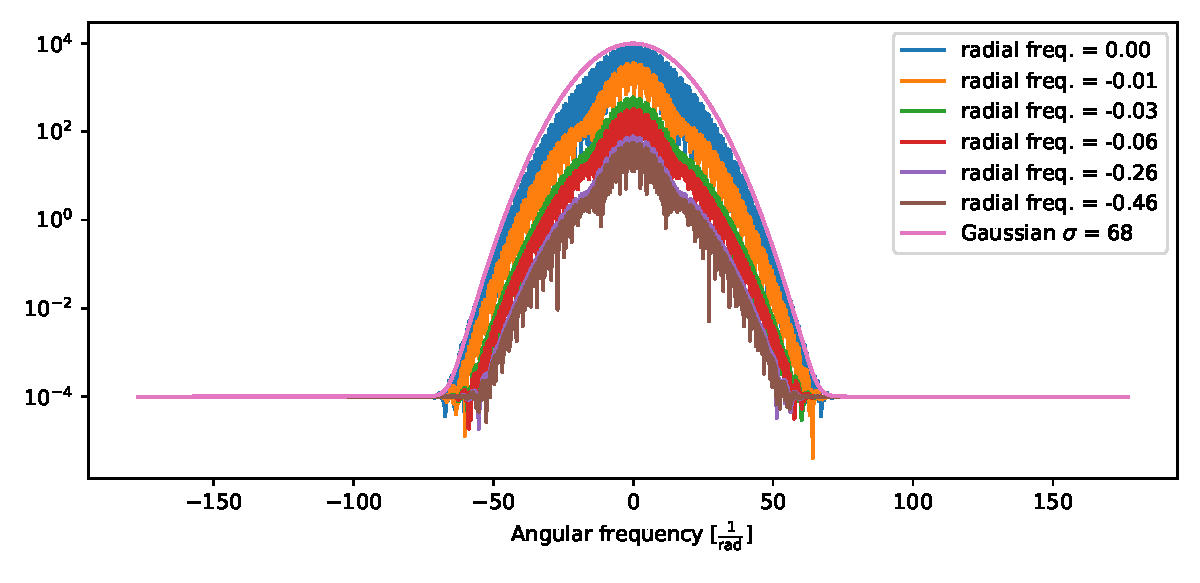
\includegraphics[width=1.0\textwidth]{pics/simspi_angularfreq.pdf}}
		\subfigure[]{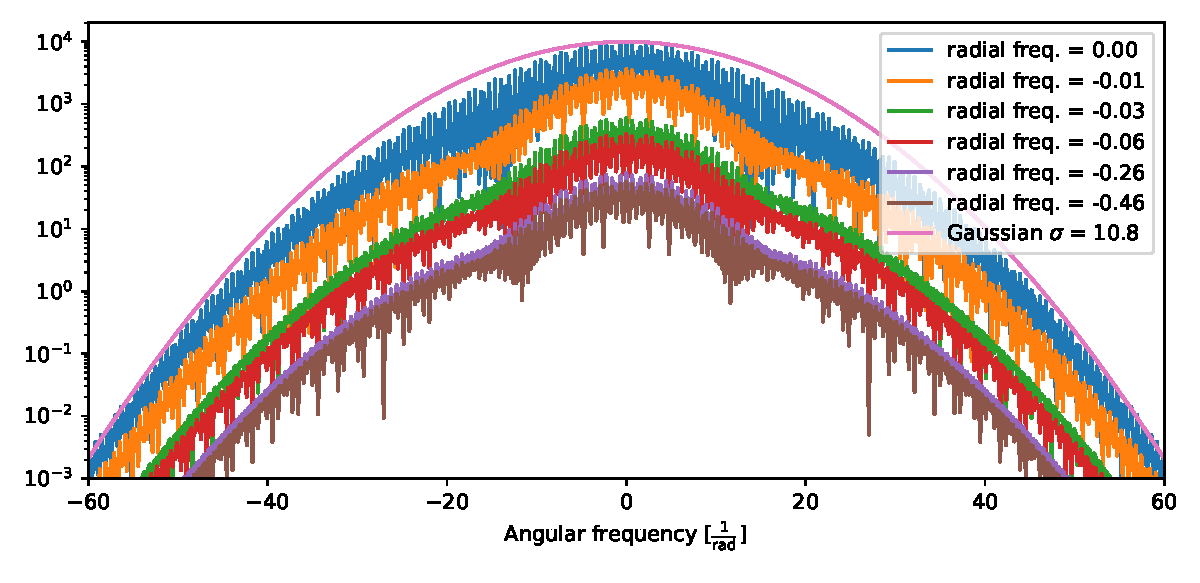
\includegraphics[width=1.0\textwidth]{pics/simspi_angularfreq_enlarged.pdf}}
\caption{The Fourier transform from figure \ref{fig:simulated_spyder} at different angular frequencies and a Gaussian profile as reference (a) and an enlarged view of it (b). }
\label{fig:simspi_angularfreq}
\end{figure}

\begin{figure}[H]
	\centering
		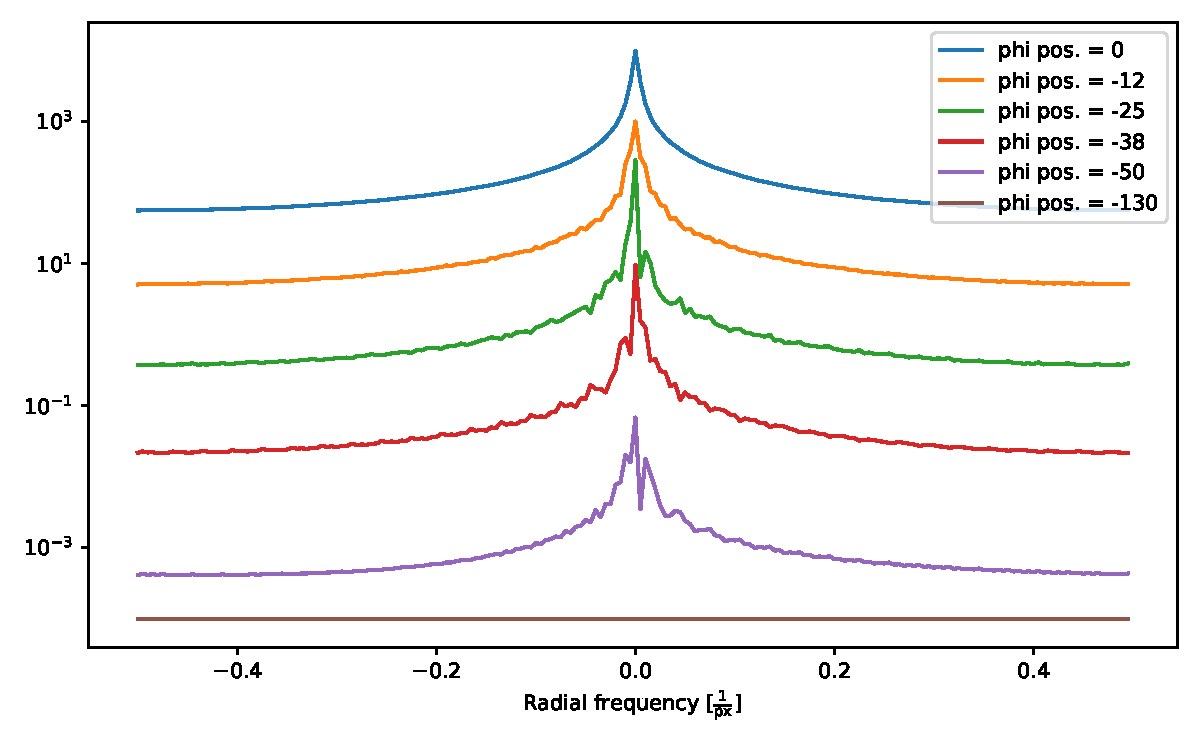
\includegraphics[width=1.0\textwidth]{pics/simspi_radialfreq.pdf}
		\caption{The Fourier transform from figure \ref{fig:simspi_radialfreq} at different radial frequencies.}
		\label{fig:simspi_radialfreq}
\end{figure}

\subsection{Noise}
\label{sec:noise}
The data will also include noise, therefore it is also important to know which effect the noise has on the Fourier transformed image. We simulate the noise by adding a random field to the simulated spider image with values between $0$ and $0.75$, since this is also about the range of the noise in our data. Figure \ref{fig:simulated_spider_noise} shows the simulated image and its frequency plane. On the first sight we see that the frequency background increased due to the noise. If we take a closer look at the intensities of the frequencies, see figure \ref{fig:simulated_spider_noise}, we find that the noisy background of the image plane produces a noisy background in the frequency plane which swallows every signal which is smaller than the noise. This means we loose a lot of information due to the noise, but this was to be expected, since this is also the effect the noise has in the image plane. Additionally the noise leads to a large increase of the intensity of the central frequency.\\
This means that due to the noise the Gaussian profile which best fits the Fourier transformation of the simulated spider at radial frequency zero is now not anymore the one with width $10.8 \frac{1}{\mathrm{rad}}$. The fit before was a good description for the bottom part of the Fourier transformation, but now this part is cut of, and the only part of the signal which is left, is the one which is mainly dominated by the widest spider. We choose a Gaussian profile of width $8.7 \frac{1}{\mathrm{rad}}$ as it is shown in figure \ref{fig:simspi_noise_angularfreq}.\\
In general we see that only the frequency close to the center are larger than the noise, such that the only radial frequencies which still can play a role are between $(-0.06, 0.06)$ $\frac{1}{\mathrm{px}}$ and the only angular frequencies are between $[-23, 23]$ $\frac{1}{\mathrm{rad}}$. This is luckily almost the same area which we before defined the be the most important. \\
We only looked at the effect randomly distributed noise has on the frequency plane, but there are also other types of noise distribution which might have a different effect. Especially the high increase of the central frequency might be different. The noisy background in the frequency plane will most probably be there also for other types of noise distributions, but the level of the background might be not distributed around a constant line, like like this is the case here or the distribution around the line is different. 
\begin{figure}[H]
	\centering
		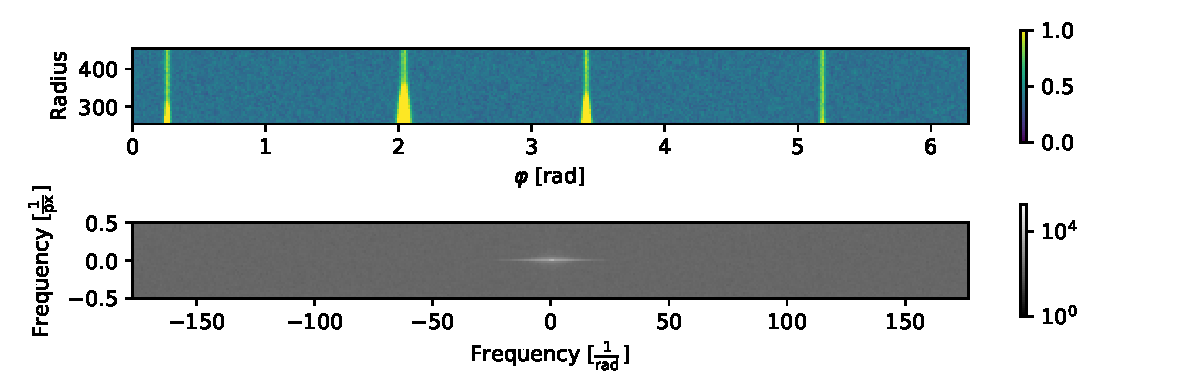
\includegraphics[width=1.0\textwidth]{pics/simulated_spider_noise.pdf}
		\caption{The image on top shows a simulation of the spiders in radius range $[254, 545]$ with a noisy background and on the bottom is the respective frequency plane.}
		\label{fig:simulated_spider_noise}
\end{figure}
\begin{figure}[H]
	\centering
		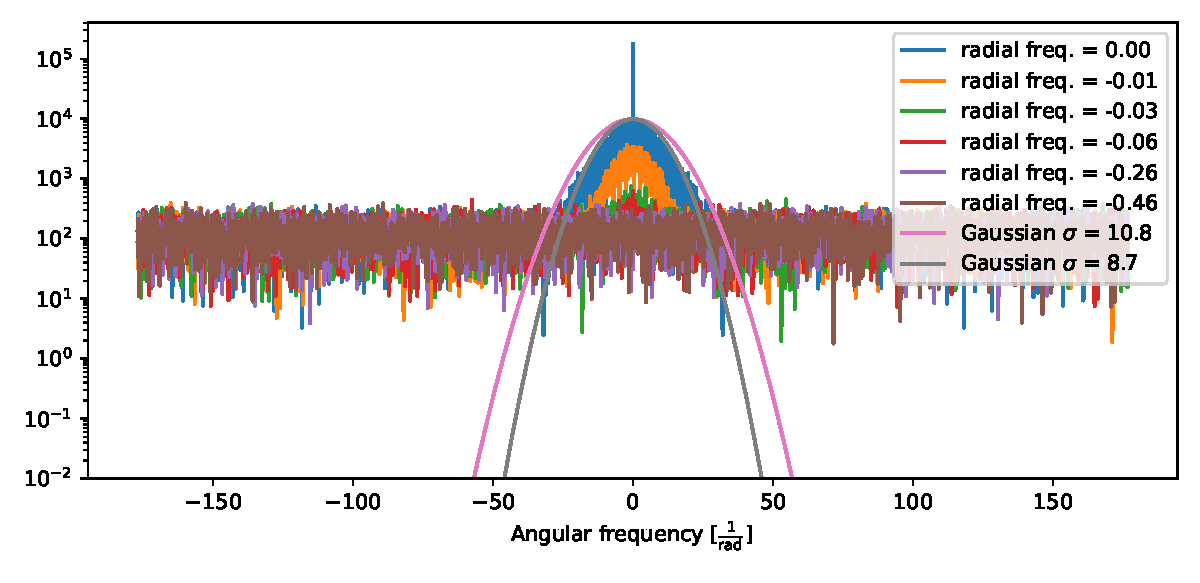
\includegraphics[width=1.0\textwidth]{pics/simspi_noise_angularfreq.pdf}
	\caption{The Fourier transform from figure \ref{fig:simulated_spider_noise} at different radial frequencies and a Gaussian profile as reference. }
\label{fig:simspi_noise_angularfreq}
\end{figure}


\subsection{Point-Like Sources}
\label{sec:pointlike}
In order to make sure that we are not going to suppress the signal of point-like sources as exoplanets we need to know how their signal is going to look like in the Fourier space.\\
We investigate the signal of a Gaussian point source and of a point spread function (PSF). A PSF describes how a point source looks like after it has gone through an imaging system \cite{PSFwiki}, which is in our case the VLT telescope with its adaptive optic. In order to simulate the PSF we use the python package AOtools \cite{AOtools}.\\
Figure \ref{fig:PSF_cut_image} shows a cut through the Gaussian and the PSF profile in the image plane. We want to compare the Fourier transformation of the PSF to the one of the Gaussian profile, of which we expect the Fourier transform to be again a Gaussian profile. The image with the PSF and its Fourier transform is shown in figure \ref{fig:PSF_fourier}. Figure \ref{fig:PSF_cut_fourier} shows the Fourier transform of a Gaussian profile and the PSF at radial frequency zero. As expected the Gaussian profile stays Gaussian in the frequency space. The Fourier transform of the PSF produces the same intensity for radial and angular frequency zero, but it decreases slower and has some local maxima. The two local maxima at each side of the global maximum produce a specific pattern which is completely different to what we get from the spiders and might be helpful to extract information about point sources from the frequency plane.  
\begin{figure}[H]
	\centering
		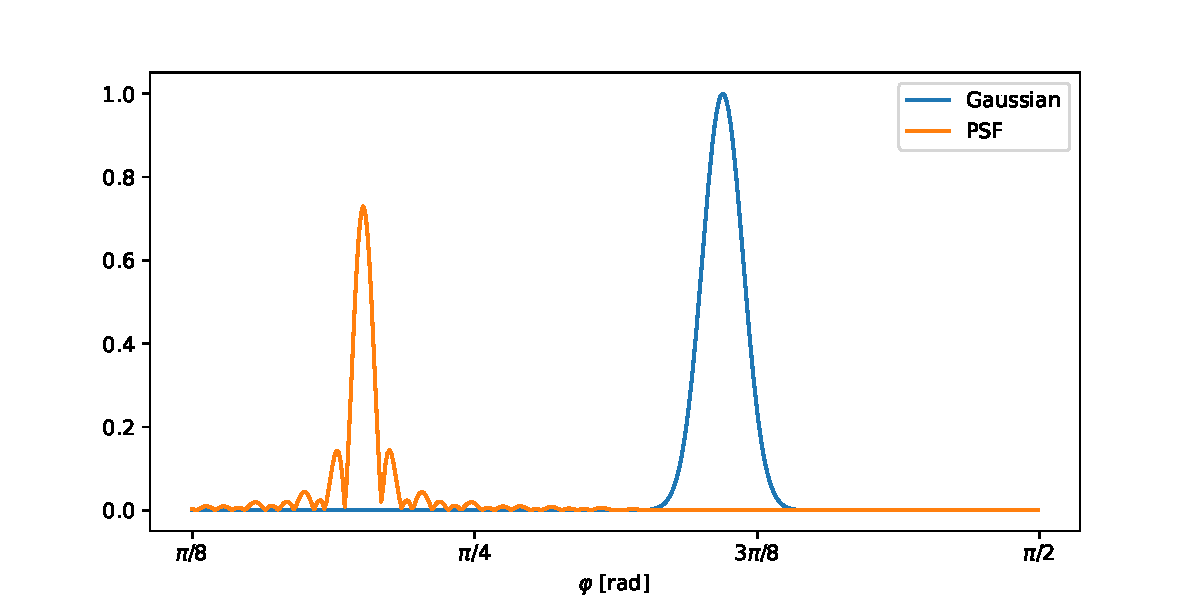
\includegraphics[width=1.0\textwidth]{pics/PSF_cut_image.pdf}
		\caption{A cut through a Gaussian profile and a PSF along the angular direction. Both profiles are rotationally symmetric.}
		\label{fig:PSF_cut_image}
\end{figure}
\begin{figure}[H]
	\centering
		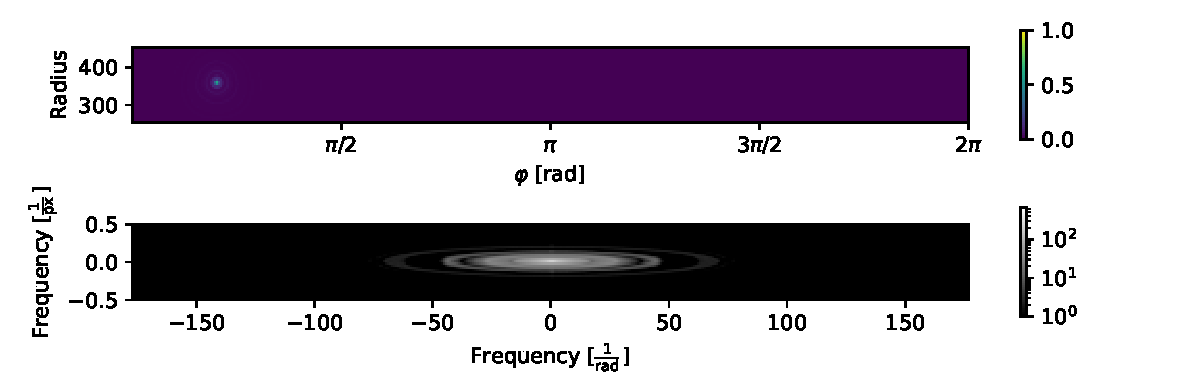
\includegraphics[width=1.0\textwidth]{pics/PSF_fourier.pdf}
		\caption{An image with a PSF (top) is transformed into the frequency space (bottom).}
		\label{fig:PSF_fourier}
\end{figure}
\begin{figure}[H]
	\centering
		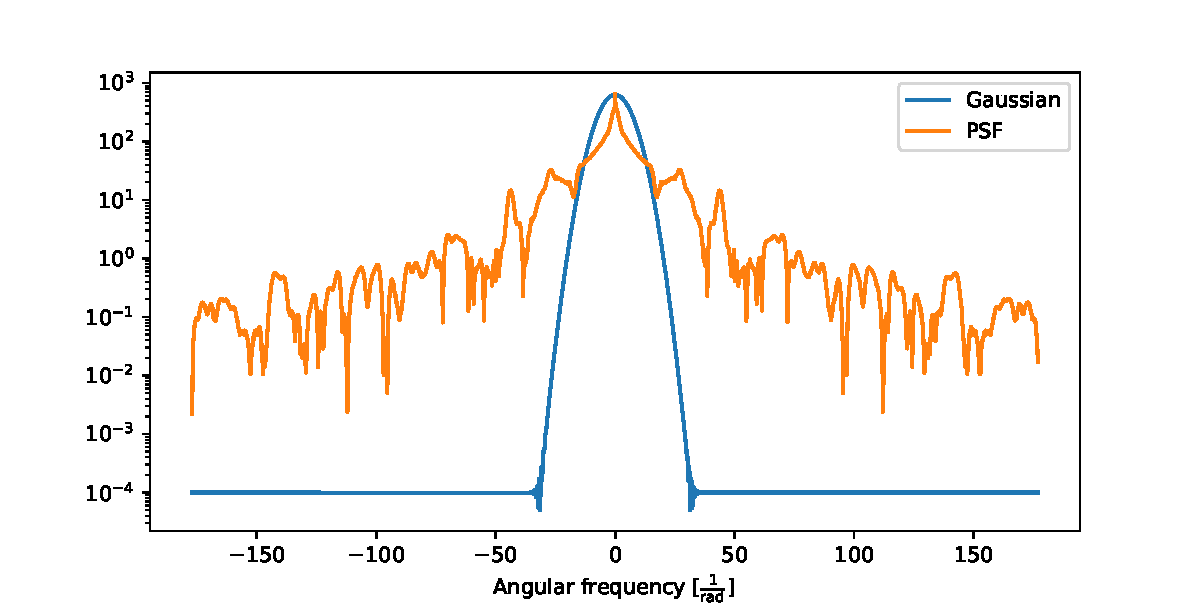
\includegraphics[width=1.0\textwidth]{pics/PSF_cut_fourier.pdf}
		\caption{The Fourier transform of a Gaussian profile and a PSF at radial frequency zero. }
		\label{fig:PSF_cut_fourier}
\end{figure}

We want to combine the knowledge about the frequency plane about the spiders with the one from the PSF. Figure \ref{fig:simulated_spyder_PSF} shows the simulated image which contains the spiders and a PSF and its Fourier transform. Figure \ref{fig:simspi_PSF_angularfreq} shows a horizontal cut through the frequency space. Since the image is an addition of the spider image and the PSF image and the Fourier transform is linear, the frequency plane should also be an addition. This is also what we see from our images. However this addition is hard to see in the logarithmic plot especially around the center frequencies. We need to keep this in mind for later, so that when we want to suppress the frequency signal from the spider, we do not accidentally subtract also signal form potential point-sources. Especially when the point-sources are really week then there frequency signals will be even weaker. 
\begin{figure}[H]
	\centering
		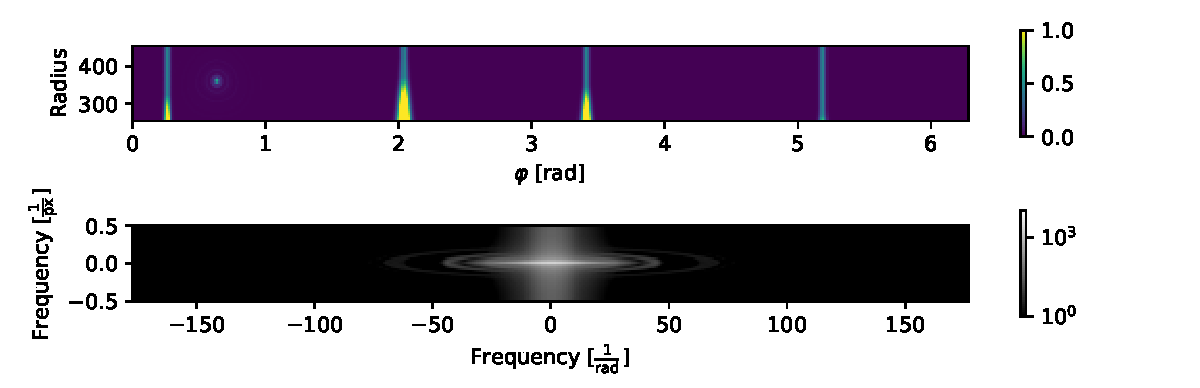
\includegraphics[width=1.0\textwidth]{pics/simulated_spyder_PSF.pdf}
		\caption{A simulation of the spiders including a PSF to simulate a point-source, like an exoplanet and the respective frequency plane.}
		\label{fig:simulated_spyder_PSF}
\end{figure}
\begin{figure}[H]
	\centering
		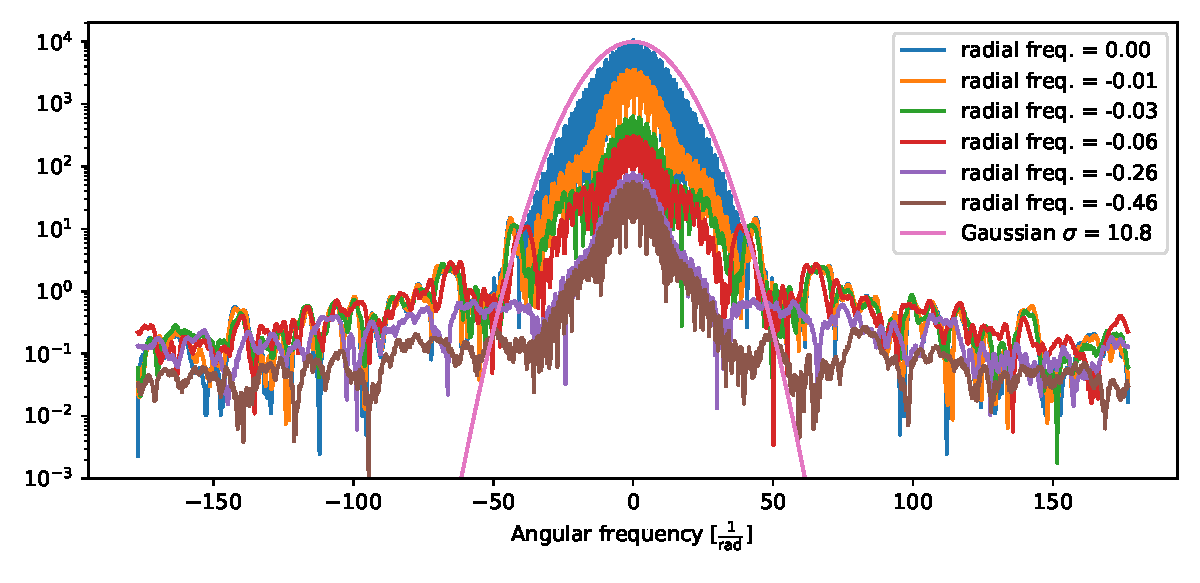
\includegraphics[width=1.0\textwidth]{pics/simspi_PSF_angularfreq.pdf}
		\caption{The Fourier transform shown in figure \ref{fig:simulated_spyder_PSF} at different radial frequencies and a Gaussian profile as reference.}
		\label{fig:simspi_PSF_angularfreq}
\end{figure}
In order to get a complete simulation from our data, we would also need to add noise to our simulation from the PSF together with the spiders. As we learned before the noise will lead to a noisy frequency background which swallows all information with a smaller intensity than the background. Therefore we need to focus on the central frequencies, which are the only ones, which are intense enough. 
\section{Suppressing the Spiders by using FFT}
We now want to use the knowledge we have gained about the Fourier transformation of different features, especially of features which resemble spiders, to suppress the signal of the spiders. The idea is to manipulate the Fourier transform of the data and then transform the data back via the inverse Fourier transformation.\\
We take the data from HD142527, warp it to the $r$-$\varphi$ plane and correct for the radial intensity drop. For the transformation we choose the radius range such that the object we want to look at is placed in the center. We choose the same radius range as in figure \ref{fig:warped_254_454} namely: $R=254-454$. In order to make sure that the aperture flux of other objects than the spiders, mainly point sources like exoplanets, is conserved we will use the ghost at radius $323$. The ghost is not perfectly in the center of the radius range, but this is not important for our purpose. The only thing which will happen, is that the aperture flux will change a bit when warping the image to the $r$-$\varphi$ plane.\\
Figure \ref{fig:rad0} shows the Fourier transform of the warped and flatten image at different radial frequencies. In contrast to the Fourier transform of the simulated spiders, the signal is not Gaussian anymore, since there are other features on top, like the ghost and the noise.
\begin{figure}[H]
	\centering
		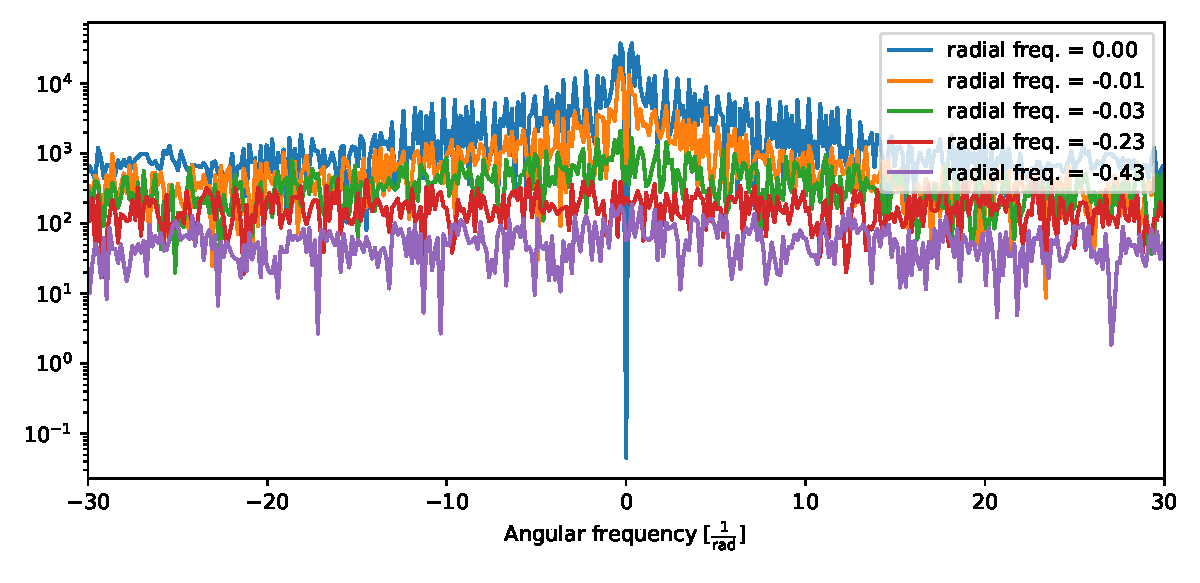
\includegraphics[width=1.0\textwidth]{pics/rad0.pdf}
		\caption{Several horizontal cuts through the frequency plane of the image data shown in figure \ref{fig:HDsuppcentralfreq_R254_R454_-0.5to0.5}(a).}
		\label{fig:rad0}
\end{figure} 

\subsection{High Frequencies}
As we saw in section \ref{sec:pointlike} the angular range in which a point-source, Gaussian or PSF, will produce a significant frequency signal is within $[-50, 50] \frac{1}{\mathrm{rad}}$ and the radial range is within $[-0.2, 0.2] \frac{1}{\mathrm{px}}$. When we consider the noise, the range is even smaller as we saw in section \ref{sec:noise}.  
Therefore we first thought it would be a good idea to suppress everything which is outside of this area by a factor of $1000$. However this is not the best idea, since the high frequencies are responsible for the edges in the image. By suppressing the high frequencies we would therefore blurry the image. This might not look like being a problem, since due to the noise the image is already blurred. As long as the point-source we look at is sufficiently large and bright this is indeed no problem, but as soon as the point-source gets fainter and smaller, it starts to disappear due to the blurring. Since we are more interested in the second case it is no option to suppress the high frequencies. Also we would not gain any positive effect through this suppression.\\
This makes us again clear that we are only looking at the absolute values of the frequency space and thus ignore big parts of the phase information as well as negative values.\\
An other attempt tried was to subtract the mean of the noisy frequency background from the whole frequency space, but this was an even badder idea. Due to the subtraction the whole back transformed image gets a weaker intensity. All structures stay unchanged, but are weaker. Like this it would be even harder to find faint structures, especially if they come too close to the numerical limits. 

\subsection{Central Radial Frequency}
\label{sec:central_radial_freq}
From our investigation of the Fourier transformation for spider-like structures, we found that their most important features are where the radial frequency is zero. Therefore, we first want to suppress the frequencies, which are caused by the spiders, at radial frequency zero.\\
As we saw in section \ref{sec:gaussian} the spiders produce a signal in the frequency plane, especially for radial frequency equals zero, which is close to a Gaussian. We divide our central radial frequency by the Gaussian profile with width $\sigma = 8.7 \frac{1}{\mathrm{rad}}$, which we found from our simulations of the spiders, see figure \ref{fig:simspi_noise_angularfreq}. By doing this we ignore the fact that we have some oscillations on top of the true signal. To reassure that this approximation is appropriate we compare the resulting back-transformed images after a division by the Gaussian profile and after a division by the Fourier transform at radial frequency zero which we get from our simulations. From the comparison we find that the Gaussian profile is a really good approximation, since by eye we cannot see any differences between the resulting back-transformed images and also the aperture fluxes of the ghosts are almost the same. We also computed the aperture flux of a PSF which we placed on the image far away from the spiders and also this aperture flux was almost the same, also for different intensities of the PSF.\\
As a next step we want to find out in which angular range around the central frequency we need to divide by the Gaussian. This is a really important parameter, since if the angular width is so large, that the value of the Gaussian profile at this position is smaller than one. The division will lead to an increase of the intensity instead of a suppression. Figure \ref{fig:rad0_diffsubwidths} shows the aperture flux of the ghost after the division by a Gaussian at radial frequency zero for different angular frequency ranges around zero. The orange line marks the aperture flux of the ghost after the warping and the correction for the radial drop-off, we call it the initial aperture flux. Whereas the blue dots mark the aperture flux of the ghost after the division by the Gaussian for different angular widths.\\
Since it is even an advantage, if the aperture flux increases through the procedure, we choose the width with which we get the largest aperture flux, which is the case for $9.1 \frac{1}{\mathrm{rad}}$. This means we divide by the Gaussian in the following angular range: $[-9.1, 9.1] \frac{1}{\mathrm{rad}}$. An increase of the aperture flux is really good, because it means that the spiders are being suppressed without suppressing the ghost. Ghost 2, at which we are looking, is a good indicator for this, because in this image he is situated close to a spider.
\begin{figure}[H]
	\centering
		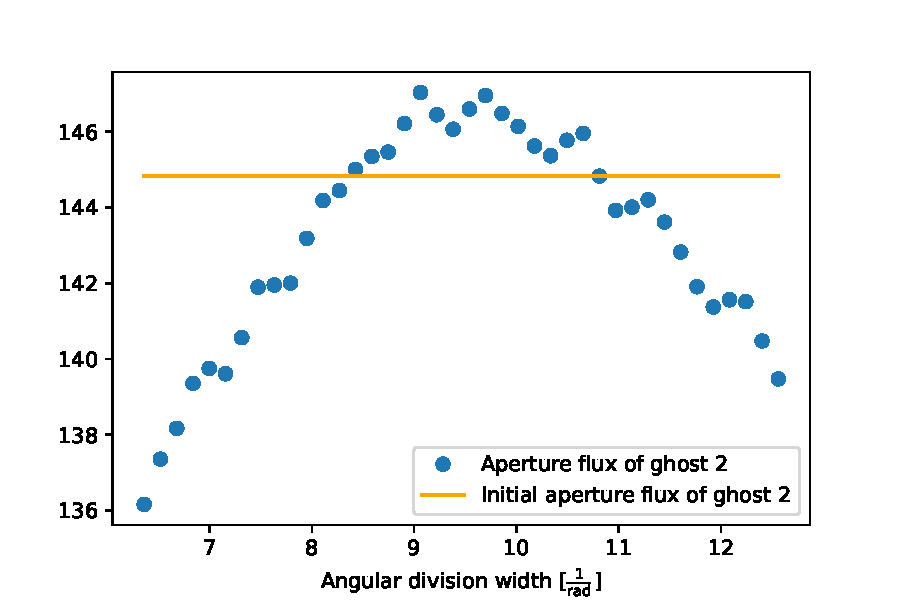
\includegraphics[width=1.0\textwidth]{pics/rad0_diffsubwidths.pdf}
		\caption{For radial frequency zero the Fourier transform of the image data is divided by a Gaussian which has its center at angular frequency zero. The division is not performed along the complete angular range, but only for a certain width around zero. We have plotted the aperture flux of ghost 2 for different angular division widths. The width which produces the largest flux is ideal.}
		\label{fig:rad0_diffsubwidths}
\end{figure}
Other parameters of this suppression are the intensity and the width of the Gaussian profile. We find that the resulting back-transformed image is not at all sensible on this variables. This is due to the fact that we divide by the Gaussian and do not subtract by it. It is not such a problem if we divide everything by $10^4$ or by $10^3$. Actually a subtraction would be mathematically more correct, but the subtraction is highly sensible on every single parameter and a division is a lot more stable. Also when dividing we can only look at the absolute values of the Fourier transform, but when subtracting we would have to take into account also the negative values. An other reason for the insensibility on the width of the Gaussian profile is that we only look at a narrow angular range, where the width of the Gaussian profile does not have a big influence. \\
Figure \ref{fig:HDsuppcentralfreq_R254_R454_-0.5to0.5}(a) shows the warped and flatten image from $R=254-454$ and its Fourier transform. In figure \ref{fig:HDsuppcentralfreq_R254_R454_-0.5to0.5}(b) the Fourier transform at radial frequency zero in the above defined angular range is divided by the Gaussian profile and its back-transformed image are shown. To get back into the $r$-$\varphi$ plane we use the inverse Fourier transformation. When we compare the image before and after the Gaussian division we can already observe that the spiders are a lot less bright. Especially around the central radius the results is really good. This is for us the most important region, since this is also the region where the object we are interested in, will be. Below the central radius the spiders almost stay the same or change only slightly and above the central radius we have a trend to the other extreme, meaning we have negative values. We also observe that the noise gets weaker and is smoother distributed.\\
From the steps we have made so far the aperture flux increases by $6.64$ \% compared to the initial aperture flux for ghost 2 and by $49.73$ \% for the PSF, here we use a PSF which is approximately $10^{-6}$ times less bright then the star. 
\begin{figure}[H]
	\centering
		\subfigure[]{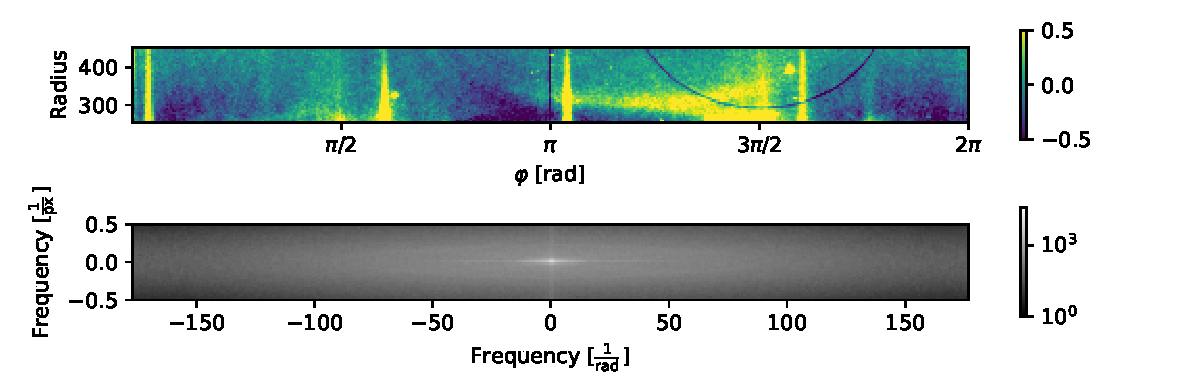
\includegraphics[width=1.1\textwidth]{pics/HDflatten_R254_R454_-0.5to0.5.pdf}}
		\subfigure[]{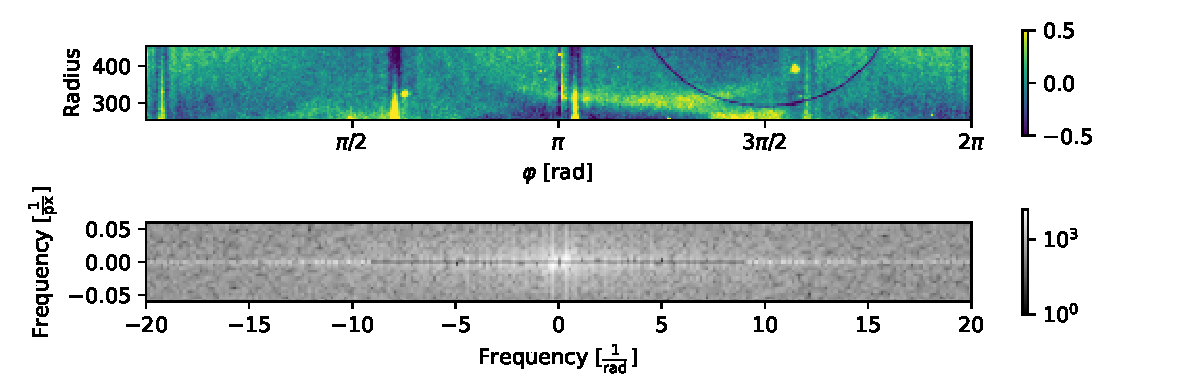
\includegraphics[width=1.1\textwidth]{pics/HDsupprcentralfreq_R254_R454_-0.5to0.5.pdf}}
\caption{An image from HD142527 which has been warped to the $r$-$\varphi$ plane and flattened and its Fourier transform (a). After a division of the central frequencies at radial frequency zero by a Gaussian profile, the spider in the back-transformed image are less bright (b).}
\label{fig:HDsuppcentralfreq_R254_R454_-0.5to0.5}
\end{figure}

\subsection{Low Frequencies}
As we saw during the simulation of the spiders, not only the frequencies at radial frequency zero have non-zero values, but there is also an extension into the radial frequencies which are unequal to zero. In the following we will also suppress the frequencies which are cause by the spiders in this regime. But due to the noise level, the interesting radial regime only goes until approximately $[-0.06, 0.06] \frac{1}{\mathrm{px}}$. As we already discussed in section \ref{sec:central_radial_freq} the regime is even smaller, since we need to avoid to divide through values which are smaller than one. The same holds for the angular range. The angular range is smaller for larger absolute radial frequency values, since the intensity of the complete signal is overall smaller. In conclusion we will only be able to suppress the lowest frequencies.\\
First of all we have to choose a Gaussian profile with an adequate width and intensity. As before when we suppressed the central radial frequency, we choose the Gaussian profiles such that it best fits to the signal of our spider simulation. For the signal at radial frequency $-0.005$/$0.005 \frac{1}{\mathrm{px}}$ (this is the one closest to the radial frequency center) we choose a Gaussian profile with width $\sigma_s = 6.4 \frac{1}{\mathrm{rad}}$ and intensity $I_s = 0.84 I = 8.4 \cdot 10^3$ where $I$ is the intensity of the Gaussian profile used for suppressing the frequencies at radius zero. As before the width and the intensity of the Gaussian profile are not so important for the suppression and does not matter if they differ a bit. But the angular frequency width $w_s$ in which we do the division (as in section \ref{sec:central_radial_freq}) as well as the radial frequency width $h$ is essential.\\
To find these two parameters we use the same procedure we used to find the angular frequency width $w$ for radial frequency zero. Namely we try out different parameters and take the one with which we get the largest aperture flux for ghost 2. As before we will also use a second object in form of a PSF which is placed not in the surrounding of one of the spiders, in order to check that the procedure really does what we want. The PSF is approximately $10^{-6}$ times less bright then the star. We find that $h = 0.01 \frac{1}{\mathrm{px}}$ and $w_s = 7.2 R \frac{1}{\mathrm{rad}}$, where $R$ is the ratio between the mean central radial frequency (considering only high angular frequencies) and the mean radial frequency in which the division is taking place.\\
Figure \ref{fig:HDsupplowfreq_R254_R454_-0.5to0.5.pdf} shows the image from HD142527 after the suppression of the low frequencies as discussed before and the suppression of the central radial frequency. We observe that now the overall brightness of each spider from figure \ref{fig:HDsuppcentralfreq_R254_R454_-0.5to0.5} to figure \ref{fig:HDsupplowfreq_R254_R454_-0.5to0.5.pdf} has not changed significantly, but the gradient from low to larger radius which we had before has almost completely vanished. Also the whole image is a lot smoother. This can also be observed in the aperture fluxes. As ghost 2 is placed near a spider and is almost in the center of the radial range, its aperture flux is almost the same as after the suppression of the central radial frequency only and so the aperture flux increased by $6.74$ \% compared to its initial aperture flux. Whereas the aperture flux of the PSF increased by $53.12$ \%. 
\begin{figure}[H]
	\centering
		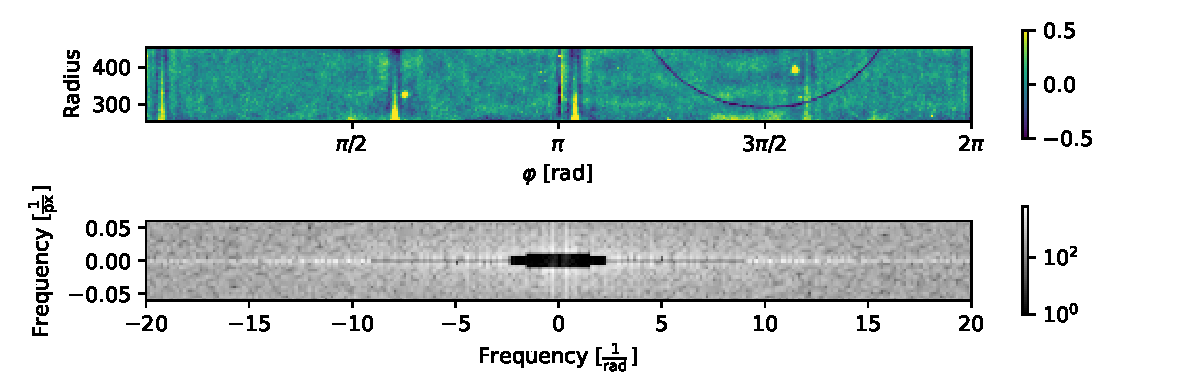
\includegraphics[width=1.1\textwidth]{pics/HDsupplowfreq_R254_R454_-0.5to0.5.pdf}
		\caption{The image from HD142527 after the central radial frequency and the low frequency are suppressed in the frequency plane and transformed back to the image plane via inverse Fourier transformation.}
		\label{fig:HDsupplowfreq_R254_R454_-0.5to0.5.pdf}
\end{figure}

\subsection{Results}
\section{Results and Discussion}
\label{sec:results}
We have seen that suppressing the spiders by subtraction in the frequency plane is not helpful, although it is mathematically correct. Due to the fact that the spiders use almost the same frequencies as potential point-sources and other important image information, we cannot simply set some frequencies to zero. We need to know how exactly the Fourier transform of the spiders look like, but when we have enough information to know the exact Fourier transform we can also simulate the spiders in the image plane and subtract it there. There is no need to go to the Fourier space. Also to do the subtraction either in the image or frequency space we assume that the spiders have a Gaussian profile and we fit this profile to the data. Doing this we risk to loose other objects which are in the same region as the spider, by accidentally subtracting them as well.\\
The suppression of the spiders by dividing by a Gaussian profile is not quite correct, however we received quite good results for the single data we have looked at in section \ref{sec:suppression}. To verify that our suppression of the spider through Gaussian division does not only work on the single data we have used until now, we perform the suppression on different images of HD142527. The data is taken in P2-mode, in this mode the ghosts and the possible exoplanets do not wander, but the spiders do. \\
Figure \ref{fig:Ghost2_apertures} (a) shows the calculated aperture flux from ghost 2 of the different images at different stages, starting with the original image, then transforming it to the $r$-$\varphi$ plane, flattening it and suppressing first the central radial frequencies and then all low frequencies. We observe that overall the aperture flux increases throughout the different steps and that it changes also during the warping due to the fact, that the ghost is not perfectly at the radial center, but it seems as if this step also slightly enhances the aperture flux. This is probably due to the fact that the ghost is in the lower part of the radial regime, so this is where, due to the warping, additional pixels need to be added which may result in an increase of the aperture flux. The flattening does not change the aperture flux much.\\
For a closer investigation on the suppression by division, we have a look at figure \ref{fig:Ghost2_apertures} (b), where we plotted the change of the aperture flux in percent and used the flattened image as reference. We observe that the suppression of the central radial frequency is the more important and the suppression of the other lower frequencies do not change much. We observe an overall increase of the aperture flux, but there are two images where the aperture flux decreased, namely at $x=3$ and $x=9$, and for the image $x=6$ the change is a lot smaller than for the rest. Here we need to keep in mind, that the position of the spiders move and that these results should depend on the distance between the ghost and the spiders. \\
We find that there are two different explanations for these cases where we have a decrease in aperture flux. One reason is that since the suppression tries to suppress the signal of the spiders, it should not change the aperture flux of the ghost, if it is not in a regime where it feels the influence of the spider. Indeed ghost 2 has the largest distance to the spiders in the image data $x=9$ and is therefore outside of the regime, where the spiders have an effect on its flux. However this result also could mean that this kind of spider suppression worsens the aperture flux a bit when we are looking at objects which are not close to any spiders.\\
An other reason for a decrease of the aperture flux (or almost no change) is that our method does not manage to suppress the spiders completely, especially in the center of the spider signal, there is no big change achieved by our suppression. This means that if the ghost and the spider overlap too much, we do not gain something from the suppression. In the image data of $x=3$ and $x=6$ the ghost is almost lying exactly on top of the spider.\\
So far we can say that the suppression by division is mainly useful if we want to find objects which are close by the spider, but not too close. This is also what we expected. We try to suppress the spiders, so our data manipulation should not have an effect on objects far away from the spiders. Also the division only makes the spiders thinner, since it corresponds to a convolution in the image plane, it will not make the spiders disappear, which means it is no help if the object lies directly behind the spider.\\
\begin{figure}[H]
	\centering
		\subfigure[]{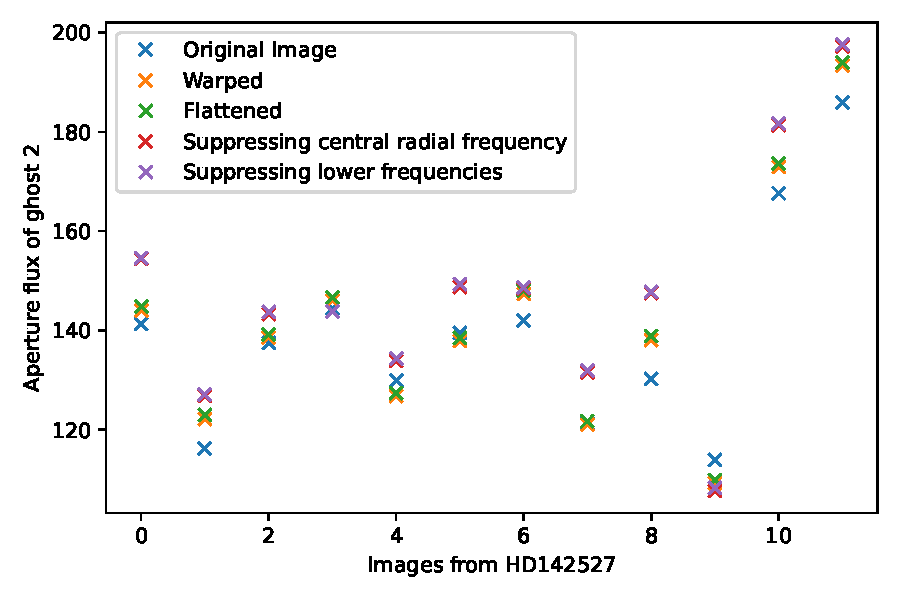
\includegraphics[width=0.49\textwidth]{pics/Ghost2_apertures.pdf}}
		\subfigure[]{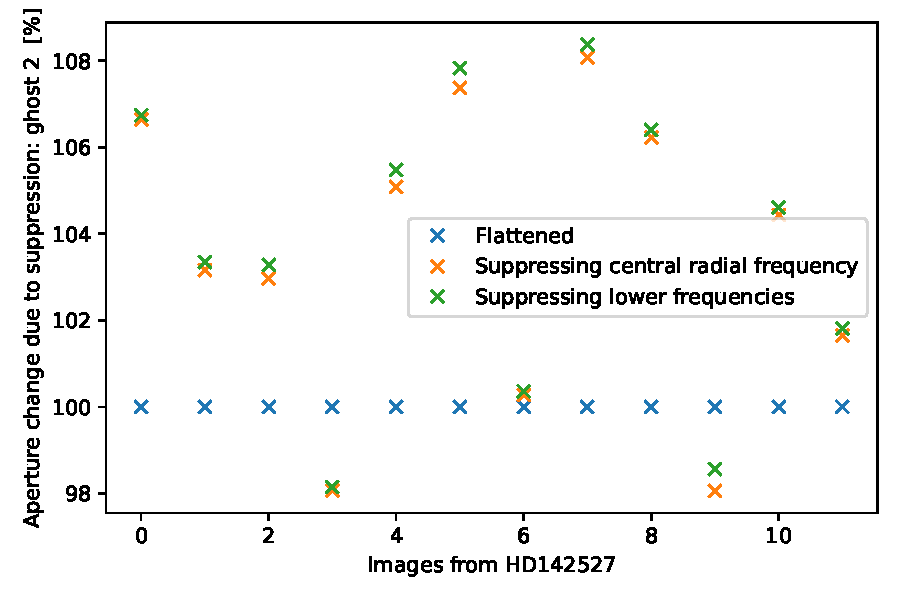
\includegraphics[width=0.49\textwidth]{pics/Ghost2_apertures_perc.pdf}}
\caption{The aperture flux of ghost 2 is calculated after each step from the transformation to the final suppression by Gaussian division (a). The aperture change due to the suppression in percent is shown in (b), where we use the flattened image as reference.}
\label{fig:Ghost2_apertures}
\end{figure}
For ghost 1 we have made the same plots as for ghost 2 which are shown in figure \ref{fig:Ghost1_apertures}. In contrast to before, where the overall aperture flux increased, we now observe a decrease in aperture flux. Mainly this decrease is caused by the warping, but this was to be expected. Since ghost 1 is in this case in the outer radial regime, pixels need to be taken together for the warping which results in a decrease of the aperture flux. Additionally the ghost gets a little bit elongated in radial direction which could also lead to a decrease in aperture flux during the suppression, since the ghost gets a form which is a little bit similar to a spider. The flattening however does not change the aperture flux much.\\
For a closer investigation on the suppression, we have a look at figure \ref{fig:Ghost1_apertures} (b). We observe that the suppression of the lower frequencies always lead to a decrease in aperture flux. The suppression of the central radial frequency mostly also leads to a decrease, only for $x=0$, $x=10$ and $x=11$ we observe an increase in aperture flux.\\
As we already observed before, the suppression only leads to an increase of the aperture flux, if the object is close enough at a spider so that it feels its influence. For the images where we observe an increase, this is also the case, whereas in all other images, the ghost is just too far away from the spiders.\\
\begin{figure}[H]
	\centering
		\subfigure[]{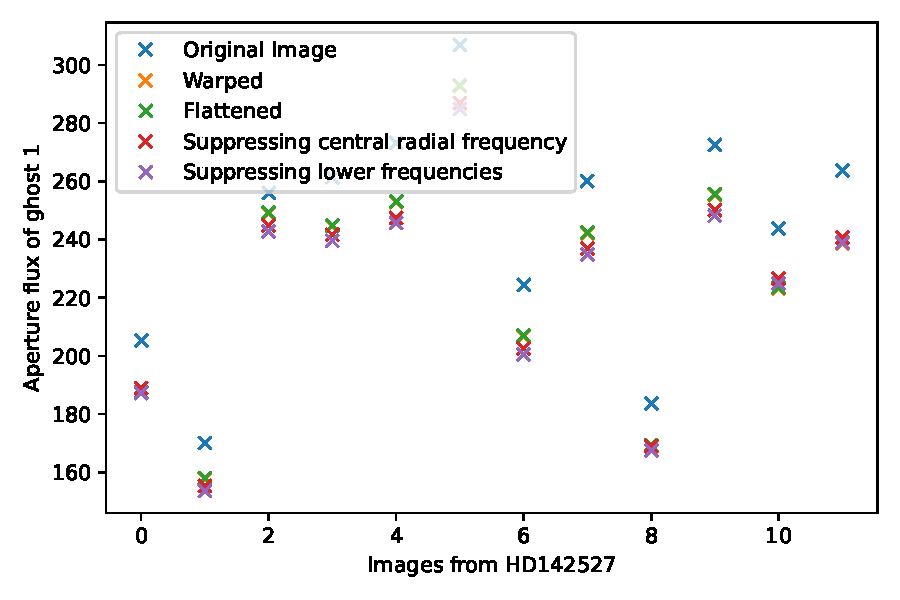
\includegraphics[width=0.49\textwidth]{pics/Ghost1_apertures.pdf}}
		\subfigure[]{\includegraphics[width=0.49\textwidth]{pics/Ghost1_apertures_perc.pdf}}
\caption{The aperture flux of ghost 1 is calculated after each step from the transformation to the final suppression by Gaussian division (a). The aperture change due to the suppression in percent is shown in (b), where we use the flattened image as reference.}
\label{fig:Ghost1_apertures}
\end{figure}
Additionally to the calculation of the aperture flux of the ghosts we have also looked at a PSF (one which is approximately $10^{-6}$ times less bright then the star). The position of the PSF is marked in figure \ref{fig:HDimg_PSF}. The chosen position of the PSF is such that in our data-set it never comes close to one of spiders. 
\begin{figure}[H]
	\centering
		\includegraphics[width=0.7\textwidth]{pics/HDimg_PSF.pdf}
		\caption{We insert a PSF into the image of HD142527. The position of the PSF is marked in the image above, where we only look at the region between $R=254-454$.}
		\label{fig:HDimg_PSF}
\end{figure}
For this PSF we also look at the same plots as we did for ghost 1 and 2. The plots are shown in figure \ref{fig:PSF1000_apertures}. We see that due to the fact that the PSF has such a low intensity the aperture fluxes are all quite small and some of them are even negative, which means that the signal of the noise is sometimes even larger than the one from the PSF. We see that the changes in aperture flux due to the different processes is actually quite small, however most of the aperture fluxes decrease a bit, especially due to the warping. Although this time the PSF is placed exactly in the center of the radius range. As before the flattening does not change the aperture flux much.\\
For a closer investigation on the suppression, we have a look at figure \ref{fig:PSF1000_apertures} (b). Here we need to be careful when we look at the percentages, since the aperture flux values are all close to zero and some even change from positive to negative values during the warping or the suppression, we observe quite large changes, when we look at the change in percentage. The aperture flux however did not change significantly. We see that we observe both increasing and decreasing fluxes which are caused by the suppression. Therefore the suppression does not seem to help for objects outside of the spiders regime. Also the smoothing of the images which we observed due to the suppression does not seem to help much. \\
\begin{figure}[H]
	\centering
		\subfigure[]{\includegraphics[width=0.49\textwidth]{pics/PSF1000_apertures.pdf}}
		\subfigure[]{\includegraphics[width=0.49\textwidth]{pics/PSF1000_apertures_perc.pdf}}
\caption{The aperture flux of a PSF is calculated after each step from the transformation to the final suppression by Gaussian division (a). The aperture change due to the suppression in percent is shown in (b), where we use the flattened image as reference.}
\label{fig:PSF1000_apertures}
\end{figure}
We find that the images which have the overall lowest brightness seem to be the one where the aperture flux increases the most during the suppression. A possible improvement would be to adjust the angular division width on the overall intensity of the image. \\
\section{Conclusion}
\label{sec:conclusion}
To suppress the spiders in astronomical data we used Fast Fourier transformation. In order to do so it is a good method to warp the image data to the $r$-$\varphi$ plane. In this plane the radial intensity structures are then all parallel to the new $y$-axis as the spider and now the radial intensity drop-off due to the star can be filtered out easily.\\
In our work we used data from HD142527 and we look at the radial regime from $R=254-454$. In this regime the two ghosts are situated, we calculated their aperture flux to check that our suppression did not accidentally filter out round objects. Additionally we also inserted a simulated PSF to investigate the effect on fainter objects. \\
We decide to suppress the spiders by dividing the low frequencies by a Gaussian profile. The advantage of the division is that we can use the Gaussian profile as an approximation for the real signal which is a lot more complicated. Additionally we can use the same intensity and width of the Gaussian profile for all images, since the suppression by division is not sensible on these parameters. However we need to limit the angular range, so that we do not divide by small numbers. An other problem of the division is that it is actually not the right approach, if we consider the theory. Dividing means that we treat the spiders as if they were a convolution on the image, but in reality they are added on top of the image data. This means that we should subtract the frequencies caused by the spiders. The problem about the subtraction is that we cannot do all these approximation, like approximating it by a Gaussian. Also the parameters are a lot more sensible and need to be chosen precisely. \\
Although the suppression by dividing the low frequencies by a Gaussian profile is theoretically not the right approach, we still receive a result, where the spiders are suppressed, at least a little and we do not loose much information about the objects at which we are interested. However the suppression only works well around the center of the chosen radius range. Also the resulting suppression is quite small, so that it is questionable if it makes sense to do it. If one decides to do suppression by division, then one should only suppress the central radial frequency, since the suppression by other frequencies does not lead to success.\\ 
It would make sense to try to suppress the spiders by subtracting certain frequencies in a future work, also if this means that one needs to determine the parameters really precisely and have individual parameters for each image data. 
 


\section{Acknowledgments}
I (Jennifer Studer) want to thank Hans Martin Schmid for is help and support I got from him during the entire project and the interesting conversation we had. For the supervision I want to thank Hans Martin Schmid and Christian Tschudi. I also want to thank Tanja Rudnicki, Tanja Finger and Kaya Ercihan for proofreading parts of my thesis. 

\newpage 

\appendix
\section{FFT of an almost Periodic Signal}
\label{almostPeriod} 
In section \ref{FFT_Lines_Beams} we have seen the Fourier transform of an image with equally spaced lines. This is a periodic pattern. But what happens if the pattern is not completely periodic anymore? By taking out one of the lines we explore the effect on the Fourier transform. In figure \ref{fig:fft_lines_almostper} we see the image, where the line which should be at $x=90$ is missing. From figure \ref{fig:fft_lines_cut_almostper} we see that the frequency spectrum still has the same shape, but the intensity range changes. The background which before was at zero (in order to plot logarithmic we added a small value) is now lifted to an intensity of $100$. 
\begin{figure}[H]
	\centering
		\includegraphics[width=1.0\textwidth]{pics/fft_simulationmorelines_almostper.pdf}
		\caption{An image with several one pixel thick lines which are almost periodically distributed on the left is transformed to the frequency plane, see image on the right.}
		\label{fig:fft_lines_almostper}
\end{figure}
\begin{figure}[H]
	\centering
		\includegraphics[width=0.8\textwidth]{pics/fft_simulation_cutmorelines_almostper.pdf}
		\caption{The intensity of the Fourier transformed image in figure \ref{fig:fft_lines_almostper} at y frequency zero.}
		\label{fig:fft_lines_cut_almostper}
\end{figure}

\newpage
\bibliographystyle{plain}
\bibliography{bib_exo}

\end{document}
